%%%%%%%%%%%%%%
%% Run LaTeX on this file several times to get Table of Contents,
%% cross-references, and citations.

%% If you have font problems, you may edit the w-bookps.sty file
%% to customize the font names to match those on your system.

%% w-bksamp.tex. Current Version: Feb 16, 2012
%%%%%%%%%%%%%%%%%%%%%%%%%%%%%%%%%%%%%%%%%%%%%%%%%%%%%%%%%%%%%%%%
%
%  Sample file for
%  Wiley Book Style, Design No.: SD 001B, 7x10
%  Wiley Book Style, Design No.: SD 004B, 6x9
%
%
%  Prepared by Amy Hendrickson, TeXnology Inc.
%  http://www.texnology.com
%%%%%%%%%%%%%%%%%%%%%%%%%%%%%%%%%%%%%%%%%%%%%%%%%%%%%%%%%%%%%%%%

%%%%%%%%%%%%%
% 7x10
%\documentclass{wileySev}

% 6x9
\documentclass{wileySix}

\usepackage{graphicx}
\usepackage{listings}

\usepackage{color}
 
\definecolor{codegreen}{rgb}{0,0.6,0}
\definecolor{codegray}{rgb}{0.5,0.5,0.5}
\definecolor{codepurple}{rgb}{0.58,0,0.82}
\definecolor{backcolour}{rgb}{0.95,0.95,0.92}
 
\lstdefinestyle{mystyle}{
    backgroundcolor=\color{backcolour},   
    commentstyle=\color{codegreen},
    keywordstyle=\color{magenta},
    numberstyle=\tiny\color{codegray},
    stringstyle=\color{codepurple},
    basicstyle=\footnotesize,
    breakatwhitespace=false,         
    breaklines=true,                 
    captionpos=b,                    
    keepspaces=true,                 
    numbers=left,                    
    numbersep=5pt,                  
    showspaces=false,                
    showstringspaces=false,
    showtabs=false,                  
    tabsize=2,
    language=sh
}
 
\lstset{style=mystyle}

%%%%%%%
%% for times math: However, this package disables bold math (!)
%% \mathbf{x} will still work, but you will not have bold math
%% in section heads or chapter titles. If you don't use math
%% in those environments, mathptmx might be a good choice.

% \usepackage{mathptmx}

% For PostScript text
\usepackage{w-bookps}

%%%%%%%%%%%%%%%%%%%%%%%%%%%%%%%%%%%%%%%%%%%%%%%%%%%%%%%%%%%%%%%%
%% Other packages you might want to use:

% for chapter bibliography made with BibTeX
% \usepackage{chapterbib}

% for multiple indices
% \usepackage{multind}

% for answers to problems
% \usepackage{answers}

%%%%%%%%%%%%%%%%%%%%%%%%%%%%%%
%% Change options here if you want:
%%
%% How many levels of section head would you like numbered?
%% 0= no section numbers, 1= section, 2= subsection, 3= subsubsection
%%==>>
\setcounter{secnumdepth}{3}

%% How many levels of section head would you like to appear in the
%% Table of Contents?
%% 0= chapter titles, 1= section titles, 2= subsection titles, 
%% 3= subsubsection titles.
%%==>>
\setcounter{tocdepth}{2}

%% Cropmarks? good for final page makeup
%% \docropmarks

%%%%%%%%%%%%%%%%%%%%%%%%%%%%%%
%
% DRAFT
%
% Uncomment to get double spacing between lines, current date and time
% printed at bottom of page.
% \draft
% (If you want to keep tables from becoming double spaced also uncomment
% this):
% \renewcommand{\arraystretch}{0.6}
%%%%%%%%%%%%%%%%%%%%%%%%%%%%%%

%%%%%%% Demo of section head containing sample macro:
%% To get a macro to expand correctly in a section head, with upper and
%% lower case math, put the definition and set the box 
%% before \begin{document}, so that when it appears in the 
%% table of contents it will also work:

\newcommand{\VT}[1]{\ensuremath{{V_{T#1}}}}

%% use a box to expand the macro before we put it into the section head:

\newbox\sectsavebox
\setbox\sectsavebox=\hbox{\boldmath\VT{xyz}}

%%%%%%%%%%%%%%%%% End Demo


\begin{document}


\booktitle{Cerdas Menguasai Git}
\subtitle{Dalam 24 Jam}

\authors{Rolly M. Awangga\\
\affil{Informatics Research Center}
%Floyd J. Fowler, Jr.\\
%\affil{University of New Mexico}
}

\offprintinfo{Cerdas Menguasai Git, First Edition}{Rolly M. Awangga}

%% Can use \\ if title, and edition are too wide, ie,
%% \offprintinfo{Survey Methodology,\\ Second Edition}{Robert M. Groves}

%%%%%%%%%%%%%%%%%%%%%%%%%%%%%%
%% 
\halftitlepage

\titlepage


\begin{copyrightpage}{2019}
%Survey Methodology / Robert M. Groves . . . [et al.].
%\       p. cm.---(Wiley series in survey methodology)
%\    ``Wiley-Interscience."
%\    Includes bibliographical references and index.
%\    ISBN 0-471-48348-6 (pbk.)
%\    1. Surveys---Methodology.  2. Social 
%\  sciences---Research---Statistical methods.  I. Groves, Robert M.  II. %
%Series.\\
%
%HA31.2.S873 2007
%001.4'33---dc22                                             2004044064
\end{copyrightpage}

\dedication{`Jika Kamu tidak dapat menahan lelahnya belajar, 
Maka kamu harus sanggup menahan perihnya Kebodohan.'
~Imam Syafi'i~}

\begin{contributors}
\name{Rolly Maulana Awangga,} Informatics Research Center., Politeknik Pos Indonesia, Bandung,
Indonesia



\end{contributors}

\contentsinbrief
\tableofcontents
\listoffigures
\listoftables
\lstlistoflistings


\begin{foreword}
Sepatah kata dari Kaprodi, Kabag Kemahasiswaan dan Mahasiswa
\end{foreword}

\begin{preface}
Buku ini diciptakan bagi yang awam dengan git sekalipun.

\prefaceauthor{R. M. Awangga}
\where{Bandung, Jawa Barat\\
Februari, 2019}
\end{preface}


\begin{acknowledgments}
Terima kasih atas semua masukan dari para mahasiswa agar bisa membuat buku ini 
lebih baik dan lebih mudah dimengerti.

Terima kasih ini juga ditujukan khusus untuk team IRC yang 
telah fokus untuk belajar dan memahami bagaimana buku ini mendampingi proses 
Intership.
\authorinitials{R. M. A.}
\end{acknowledgments}

\begin{acronyms}
\acro{AI}{Artificial Intelligence}
\acro{ETL}{Extract Transform Load}
\acro{NLP}{Natural Language Processing}

\end{acronyms}

\begin{glossary}
\term{git}Merupakan manajemen sumber kode yang dibuat oleh linus torvald.

\term{bash}Merupakan bahasa sistem operasi berbasiskan *NIX.

\term{linux}Sistem operasi berbasis sumber kode terbuka yang dibuat oleh Linus Torvald
\end{glossary}

\begin{symbols}
\term{A}Amplitude

\term{\hbox{\&}}Propositional logic symbol 

\term{a}Filter Coefficient

\bigskip

\term{\mathcal{B}}Number of Beats
\end{symbols}

\begin{introduction}

%% optional, but if you want to list author:

\introauthor{Rolly Maulana Awangga, S.T., M.T.}
{Informatics Research Center\\
Bandung, Jawa Barat, Indonesia}

Pada era disruptif  \index{disruptif}\index{disruptif!modern} 
saat ini. git merupakan sebuah kebutuhan dalam sebuah organisasi pengembangan perangkat lunak.
Buku ini diharapkan bisa menjadi penghantar para programmer, analis, IT Operation dan Project Manajer.
Dalam melakukan implementasi git pada diri dan organisasinya.

Rumusnya cuman sebagai contoh aja biar keren\cite{awangga2018sampeu}.

\begin{equation}
ABC {\cal DEF} \alpha\beta\Gamma\Delta\sum^{abc}_{def}
\end{equation}

\end{introduction}

%%%%%%%%%%%%%%%%%%Isi Buku_

\chapter{Pengenalan Kecerdasan Buatan dan Scikit-Learn}
\section{Kecerdasan Buatan}
\subsection{Definisi Kecerdasan Buatan}
    Kecerdasan Buatan biasa disebut dengan istilah AI (Artificial Intelligence). AI sendiri merupakan suatu cabang dalam bisnis sains komputer sains dimana mengkaji tentang bagaimana cara untuk menlengkapi sebuah komputer dengan kemampuan atau kepintaran layaknya atau mirip dengan yang dimiliki manusia. Sebagai contoh, sebagaimana komputer dapat berkomunikasi dengan pengguna baik menggunakan kata, suara maupun lain sebagainya. Dengan kemampuan ini, diharapkan komputer mampu mengambil keputusan sendiri untuk berbagai kasus yang ditemuinya kemudian itulah yang disebut dengan kecerdasan buatan. Kecerdasan buatan adalah kemampuan komputer digital atau robot yang dikendalikan konputer untuk melakukan tugas yang umumnya dikaitkan dengan sesuatu yang cerdas. Istilah ini sering diterapkan pada proyek pengembangan sistem yang diberkahi dengan karakteristik proses intelektual manusia, seperti kemampuan untuk berpikir, menemukan makna, menggeneralisasi, atau belajar dari pengalaman masa lalu.

    Kecerdasan Buatan adalah salah satu bidang studi yang berhubungan dengan pemanfaatan mesin untuk memecahkan persoalan yang rumit dengan cara lebih manusiawi dan lebih bisa di pahami oleh manusia. Kecerdasan buatan makin canggih dengan kemampuan komputer dalam memperbarui pengetahuannya dengan banyaknya testing dan perkembangan target analisa. Untuk kecerdasan buatan ada banyak contoh dan jenisnya. Salah satu contoh yang paling terkenal dari Artificial Intelligence ialah Google Assistant. Google Assistant digunakan untuk kemudahan user dalam menemukan berbagai hal maupun penyetingan langsung terhadap smartphone yang digunakan dan masih banyak lagi.

\subsection{Sejarah Kecerdasan Buatan}
    Artificial intelligence merupakan inovasi baru di bidang ilmu pengetahuan. Mulai terbentuk sejak adanya komputer modern dan kira-kira terjadi sekitaran tahun 1940 dan 1950. Ilmu pengetahuan komputer ini khusus ditujukan dalam perancangan otomatisasi tingkah laku cerdas dalam sistem kecerdasan komputer. Pada awal 50-an, studi tentang “mesin berpikir” memiliki berbagai nama seperti cybernetics, teori automata, dan pemrosesan innformasi. Pada tahun 1956, para ilmuan jenius seperti Alan Turing, Norbert, Wiener, Claude Shannon dan Warren McCullough telah bekerja secara independen dibidang cybernetics, matematika, algoritma dan teori jaringan. Namun, seprang ilmuan komputer dan kognitif John McCarthy adalah orang yang dating dengan ide untuk bergabung dengan upaya penelitian terpisah ini kedalam satu bidang yang akan mempelajari topic baru untuk imajinasi manusia yaitu kecerdasan buatan. Dia adalah orang yang menciptakan istilah tersebut dan kemudian mendirikan laboratorium Kecerdasan Buatan di MIT dan Stan ford.

    Pada tahun 1956, McCarthy yang sama mendirikan Konferensi Dartmouth di Hanover, New Hampshire. Peneliti terkemuka dalam teori kompleksitas, simulasi bahasa, hubungan antara keacakan dan pemikiran kreatif, jaringan saraf diundang. Tujuan dari bidang penelitian yang baru dibuat adalah untuk mengembangkan mesin yang dapat mensimulasikan setiap aspek kecerdasab. Itulah sebabnya Konferensi Dartmouth 1956 dianggap sebagai kelahiran Kecerdasan Buatan. Sejak saat itu, Kecerdasa Buatan telah hidup melalui decade kemuliaan dan cemoohan, yang dikenal luas sebagai musim panas dan musim dingin AI. Musim panasnya ditandai dengan optimism dan dana besar, sedangkan musim dinginnya dihadapkan dengan pemotongan dana, ketidakkpercayaan dan pesimisme.

\subsection{Perkembangan Kecerdasan Buatan}
    Teknologi Artificial Intelligence semakin ramai dibahas dalam berbagai diskusi teknologi di seluruh dunia.Menurut kebanyakan orang, pekerjaan seperti kasir, operator telepon, pengendara truk, dan lainnya sangat berpeluang besar untuk tergantikan oleh Artificial Intelligence. Mengapa terjadi hal demikian? dikarenakan memang bahwa AI lebih ungul dalam hal kinerja, fitur dan lain sebagainya. Namun, dalam beberapa aspek memang pekerja manusia masih unggul dibandingkan AI itu sendiri. Para generasi muda yang ada di dunia terutama di daerah Asia terlihat sudah memahami fungsi dan efek dari AI dalam kehidupan kita sehari-hari. Berdasarkan survei yang dilakukan oleh Microsoft, terdapat 39 persen responden yang mempertimbangkan untuk menggunakan mobil tanpa pengemudi dan 36 persen lainnya setuju bahwa robot masa depan dengan software untuk beroperasi mampu meningkatkan produktivitas. Dari survey tersebut kita sebagai pengguna AI harus lebih bijaksana dalam pengembangan dan penggunaan dari AI sehingga tanpa memberikan efek samping terhadap etos kerja dan keseharian kita sebagai pengguna dalam kehidupan sehari-hari.

    AI Summer 1 (1956-1973) KOnferensi Dartmounth diikuti oleh 17 tahun kemajuan luar biasa. Proyek penelitian yang dilakukan di MIT, universitas di Edinburgh, Stanford dan Carnegie Mellon menerima dana besar-besaran, yang akhirnya membuahkan hasil. Selama tahun-tahun itulah komputer pemrograman mulai melakukan masalah aljabar, membuktikan teorema geometris, memahami dan menggunakan sintaks dan tata bahasa Inggris. Terlepas dari ditinggalkannya koneksionisme dan terjemahan mesin yang gagal, yang menunda penelitian Natural Language Processing (NLP) selama bertahun-tahun, banyak prestasi dari masa lalu yang membuat sejarah. Berikut ini beberapa diantaranya : Pelopor pembelajaran mesin, Ray Solomonoff meletakkan dasar-dasar teori metematika AI, memperkenalkan metode Bayesian universal untuk inferensi dan preddiksi induktif Thomas Evans menciptakan program ANALOGI heuristik, yang memungkinkan komputer memecahkan masalah geometri-analogi Unimation, perusahaan robotika pertma didunia, menciptakan robot industri Unimate, yang bekerja pada jalur perakitan modil Genenral Motors. Joseph Weizenbaum membangun ELIZA-program interaktif yang dapat membawa percakapan dalam bahasan Inggris tentang topik apapun. Ross Quillian menunjukkan jaring semanik, sedangkan Jaime Carbonell (Sr.) mengembangkan Cendikia-program interaktif untuk instruksi yang dibantu komputer berdasarkan jaring semantik. Edward Feigenbaum dan Julian Feldman menerbitkan Computeks and Thought, kumpulan artikel pertama tentang AI.

\section{Scikit-Learn}
\subsection{Supervised Learning}
Supervised Learning adalah tugas pengumpulan data untuk menyimpulkan fungsi dari data pelatihan berlabel. Data pelatihan terdiri dari serangkaian contoh pelatihan. Dalam supervised learning, setiap contoh adalah pasangan yang terdiri dari objek input (biasanya vektor) dan nilai output yang diinginkan(juga disebut sinyal pengawasan super). Algoritma pembelajaran yang diawasi menganalisis data pelatihan dan menghasilkan fungsi yang disimpulkan, yang dapat digunakan untuk memetakan contoh-contoh baru. Skenario optimal akan memungkinkan algoritma menentukan label kelas dengan benar untuk instance yang tidak terlihat. Ini membutuhkan algoritma pembelajaran untuk menggeneralisasi dari data pelatihan untuk situasi yang tidak terlihat dengan cara yang "masuk akal". Supervised Learning adalah pendekatan dimana sudah terdapat data yang dilatih selain itu juga terdapat variable yang ditargetkan sehingga tujuan dari pendekatan ini yaitu mengelompokkan suatu data ke dta yang sudah ada. Supervised Learning menyediakan algoritma pembelajaran dengan jumlah yang diketahui untuk mendukung penilaian dimasa depan. Chatbots, mobil self-driving, program pengenalan wajah, sistem pakar dan robot adalah beberapa sistem yang dapat menggunakan pembelajaran yang diawasi atau tidak diawasi. Supervised Learning sebagian besar terkait dengan AI berbasis pengambilan tetapi mereka juga mungkin mampu menggunakan model pembelajaran generatif. Data pelatihan untuk pembelajaran yang diawasi mencakup serangkaian contoh dengan subjek input berpasangan dan output yang diinginkan (yang juga disebut sebagai sinyal pengawasan).

Dalam pembelajaran yang diawasi untuk pemrosesan gambar, misalnya sistem AI mungkin dilengkapi dengan gambar berlabel kendaraan dalam ketegori seperti mobil dan truk. Setelah jumlah pengamatan yang cukup, sistem harus dapat membedakan antara dan mengkategorikan gambar yang tidak berlabel, dimana waktu pelatihan dapat dikatakan lengkap. Model Supervised Learning memiliki beberapa keunggulan dibandingkan pendekatan tanpa pengawasan, tetapi mereka juga memiliki keterbatasan. Sistem lebih cenderung membuat penilaian bahwa manusia dapat berhubungan, misalnya karena manusia telah memberikan dasar untuk keputusan. Namun, dalam kasus metode berbasis pengambilan, Supervised Learning mengalami kesulitan dalam menangani informaasi baru. Jika suatu sistem dengan kategori untuk mobil dan truk disajikan dengan sepeda, misalnya ia harus salah dikelompokkan dalam satu kategori ata yang lain. Namun. jika sistem AI bersifat generatif, ia mungkin tidak tahu apa sepeda itu tetapi akan dapat mengenalinya sebagai milik kategori yang terpisah.

\subsection{Regresi}
Regresi adalah metode analisis statistik yang digunakan untuk melihat pengaruh antara dua ataupun lebih variabel. Regresi adalah membahas masalah ketika variabel output adalah nilai riil atau berkelanjutan, seperti "gaji" atau "berat". Banyak model yang berbeda dapat digunakan makan, yang paling sederhana adalah regresi linier. Ia mencoba untuk menyesuaikan data dengan hyper-plane terbaik yang melewati poin.

\subsection{Klasifikasi}
Klasifikasi adalah pembagian sesuatu menurut kelas-kelas ( class ). Menurut Ilmu Pengetahuan, Klasifikasi merupakan proses pengelompokkan benda berdasarkan ciri-ciri persamaan dan juga perbedaan. Dalam masalah klasifikasi, kami mencoba memprediksi sejumlah nilai terpisah. Label (y) umumnya datang dalam bentuk kategorikal dan mewakili sejumlah kelas. Dalam pembelajaran mesin dan statistik, klasifikasi adalah pendekatan pembelajaran yang diawasi di mana program komputer belajar dari input data yang diberikan kepadanya dan kemudian menggunakan pembelajaran ini untuk mengklasifikasikan pengamatan baru. Kumpulan data ini mungkin hanya bersifat dua kelas (seperti mengidentifikasi apakah orang tersebut berjenis kelamin laki-laki atau perempuan atau bahwa surat itu spam atau bukan-spam) atau mungkin juga multi-kelas. Beberapa contoh masalah klasifikasi adalah: pengenalan ucapan, pengenalan tulisan tangan, identifikasi metrik, klasifikasi dokumen dll.

\subsection{Unsupervised Learning}
Unsupervised Learning berbeda dengan Supervised Leraning. Perbedaannya ialah unsupervised learning tidak memiliki data latih, sehingga dari data yang ada kita mengelompokan data tersebut menjadi 2 ataupun 3 bagian dan seterusnya. Unsupervised Learning adalah pelatihan algoritma kecerdasan buatan (AI) menggunakan informasi yang tidak diklasifikasikan atau diberi label dan memungkinkan algoritma untuk bertindak atas informasi tersebut tanpa bimbingan. Dalam Unsupervised Learning, sistem AI dapat mengelompokkan informasi yang tidak disortir berdasarkan persamaan dan perbedaan meskipun tidak ada kategori yang disediakan.

Dalam Unsupervised Learning, sistem AI disajikan dengan data yang tidak berlabel, tidak terkategorisasi dan algoritma sistem bekerja pada data tanpa pelatihan sebelumnya. Outputnya tergantung pada algoritma kode. Menundukkan suatu sistem pada Unsupervised Learning adalah salah satu cara untuk menguji AI. Algoritma Unsupervised Learning dapat melakukan tugas pemrosesan yang lebih kompleks daripada sistem pembelajaran yang
diawasi. Namun, pembelajaran tanpa pengawasan bisa lebih tidak terduga daripada model alternatif. Sementara Unsupervised Learningi mungkin, misalnya, mencari tahu sendiri cara memilah kucing dari anjing, mungkin juga menambahkan kategori yang tidak terduga dan tidak diinginkan untuk menangani breed yang tidak biasa, membuat kekacauan bukannya keteraturan

\subsection{Data Set}
Dataset adalah objek yang merepresentasikan data dan juga relasi yang ada di memory. Strukturnya mirip dengan data di database, namun bedanya
dataset berisi koleksi dari data table dan data relation. mendapatkan data yang tepat berarti mengumpulkan atau mengidentifikasi data yang berkorelasi dengan hasil yang ingin Anda prediksi; yaitu data yang berisi sinyal tentang peristiwa yang Anda pedulikan. Data harus diselaraskan dengan masalah yang Anda coba selesaikan. Gambar kucing tidak terlalu berguna ketika Anda sedang membangun sistem identifikasi wajah. Memverifikasi bahwa data selaras dengan masalah yang ingin Anda selesaikan harus dilakukan oleh ilmuwan data. Jika Anda tidak memiliki data yang tepat, maka upaya Anda untuk membangun solusi AI harus kembali ke tahap pengumpulan data. Format ujung kanan untuk pembelajaran dalam umumnya adalah tensor, atau array multi-dimensi. Jadi jalur pipa data yang dibangun untuk pembelajaran mendalam umumnya akan mengkonversi semua data - baik itu gambar, video, suara, suara, teks atau deret waktu  menjadi vektor dan tensor yang dapat diterapkan operasi aljabar linier. Data itu seringkali perlu dinormalisasi, distandarisasi dan dibersihkan untuk meningkatkan kegunaannya, dan itu semua adalah langkah dalam ETL pembelajaran mesin. Deeplearning4j menawarkan alat ETV DataVec untuk melakukan tugas-tugas pemrosesan data tersebut.

Pembelajaran yang dalam, dan pembelajaran mesin yang lebih umum, membutuhkan pelatihan yang baik agar bekerja dengan baik. Mengumpulkan dan membangun set pelatihan  badan yang cukup besar dari data yang diketahui  membutuhkan waktu dan pengetahuan khusus domain tentang di mana dan bagaimana mengumpulkan informasi yang relevan. Perangkat pelatihan bertindak sebagai tolok ukur terhadap mana jaring pembelajaran dalam dilatih. Itulah yang mereka pelajari untuk direkonstruksi sebelum mereka melepaskan data yang belum pernah mereka lihat sebelumnya. Pada tahap ini, manusia yang berpengetahuan luas perlu menemukan data mentah yang tepat dan mengubahnya menjadi representasi numerik yang dapat dipahami oleh algoritma pembelajaran mendalam, tensor. Membangun set pelatihan, dalam arti tertentu, pra-pra pelatihan. Set pelatihan yang membutuhkan banyak waktu atau keahlian dapat berfungsi sebagai keunggulan dalam dunia ilmu data dan pemecahan masalah. Sifat keahlian sebagian besar dalam memberi tahu algoritma Anda apa yang penting bagi Anda dengan memilih apa yang masuk ke dalam set pelatihan. Ini melibatkan menceritakan sebuah kisah  melalui data awal yang Anda pilih yang akan memandu jaring pembelajaran mendalam Anda saat mereka mengekstraksi fitur-fitur penting, baik di set pelatihan maupun dalam data mentah yang telah mereka ciptakan untuk dipelajari. Untuk membuat set pelatihan yang bermanfaat, Anda harus memahami masalah yang Anda selesaikan; yaitu apa yang Anda inginkan agar jaring pembelajaran mendalam Anda memperhatikan, di mana hasil yang ingin Anda prediksi.

\subsection{Training Set}
Training Set adalah set digunakan oleh algoritma klassifikasi . Dapat dicontohkan dengan : decision tree, bayesian, neural network dll. Semuanya dapat digunakan untuk membentuk sebuah model classifier. Menjalankan pelatihan yang diatur melalui jaringan saraf mengajarkan pada net
cara menimbang berbagai fitur, menyesuaikan koefisien berdasarkan kemungkinan mereka meminimalkan kesalahan dalam hasil Anda. Koefisien-koefisien tersebut, juga dikenal sebagai parameter, akan terkandung dalam tensor dan bersama-sama mereka disebut model, karena mereka mengkodekan model data yang mereka latih. Mereka adalah takeaways paling penting yang akan Anda dapatkan dari pelatihan jaringan saraf.

\subsection{Testing Set}
Testing Set adalah set yang digunakan untuk mengukur sejauh mana classifier berhasil melakukan klasifikasi dengan benar. Ini berfungsi sebagai meterai persetujuan, dan Anda tidak menggunakannya sampai akhir. Setelah Anda melatih dan mengoptimalkan data Anda, Anda menguji jaringan saraf Anda terhadap pengambilan sampel acak akhir ini. Hasil yang dihasilkannya harus memvalidasi bahwa jaring Anda secara akurat mengenali gambar, atau mengenalinya setidaknya [x] dari jumlah tersebut. Jika Anda tidak mendapatkan prediksi yang akurat, kembalilah ke set pelatihan, lihat hyperparameter yang Anda gunakan untuk menyetel jaringan, serta kualitas data Anda dan lihat teknik pra-pemrosesan Anda.

\section{Instalasi dan Pemakaian Scikit-Learn}
\subsection{Instalasi library scikit dari anaconda, mencoba kompilasi dan uji coba ambil contoh kode dan lihat variabel explorer}
\begin{enumerate}
\item Pastikan bahwa sudah terinstal Anaconda pada PC anda, caranya buka CMD lalu ketikan \textit{conda --version} jika hasilnya seperti
\begin{figure}
	\begin{center}
   	 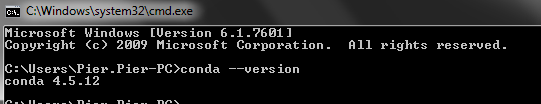
\includegraphics[scale=0.5]{figures/versiconda.png}
   	 \caption{Versi Anaconda Yang Digunakan}	
	\end{center}
\end{figure}

\item Pastikan juga Kebutuhan Scikit seperti Numpy, Scipy dan Python telah terinstal. untuk mengeceknya buka CMD dan ketikan seperti gambar berikut.
\begin{figure}
	\begin{center}
   	 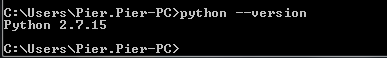
\includegraphics[scale=0.5]{figures/gambar.png}
   	 \caption{Versi Python Yang Digunakan}	
	\end{center}
\end{figure}

\item Pada CMD ketikan \textit{conda install scikit-learn} kemudian tunggu sampai instalasi selesai.
\begin{figure}[!htbp]
	\begin{center}
   	 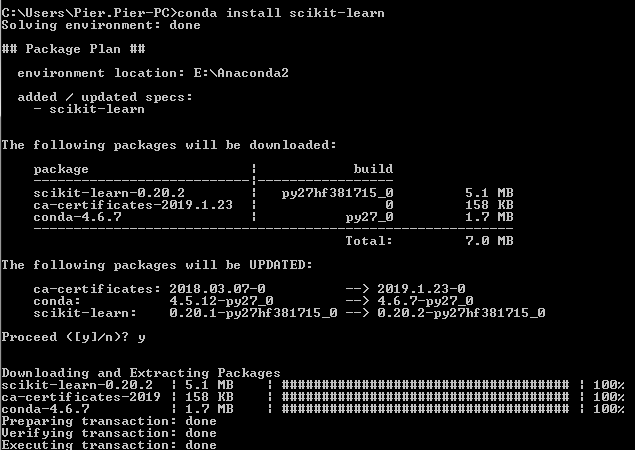
\includegraphics[scale=0.5]{figures/instalscikit.png}
   	 \caption{Instalasi Scikit Dari Anaconda}	
	\end{center}
\end{figure}

\item Setelah itu, kita akan mencoba salah satu contoh dasar penggunaan scikit pada website sebelumnya. Dan disini menggunakan contoh Multilabel classification.
\item Salin skrip contoh tersebut ke Text Editor Visual Code atau yang anda miliki. File ini kemudian di save dengan nama `contoh.py'
\begin{figure}
	\begin{center}
   	 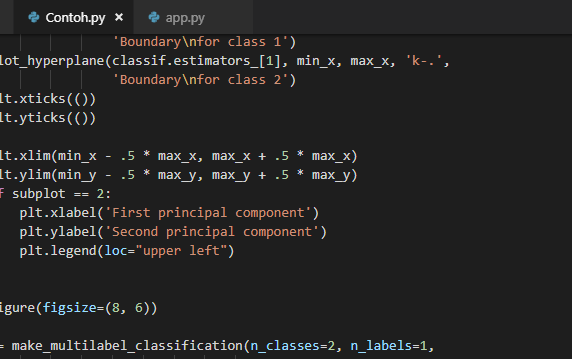
\includegraphics[scale=0.5]{figures/contoh.png}
   	 \caption{Contoh Skrip}	
	\end{center}
\end{figure}
\item Setelah tersimpan, jalankan di CMD dengan mengetikan `python contoh.py' maka akan muncul hasil seperti dibawah ini.
\begin{figure}
	\begin{center}
   	 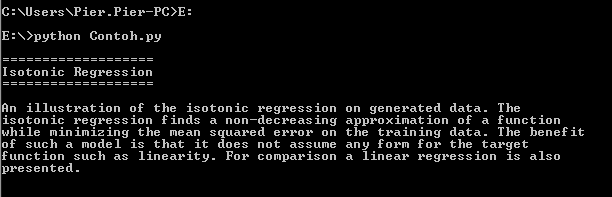
\includegraphics[scale=0.5]{figures/hasil1.png}
   	 \caption{Hasil Yang Muncul Di CMD}	
	\end{center}
\end{figure}

\begin{figure}
	\begin{center}
   	 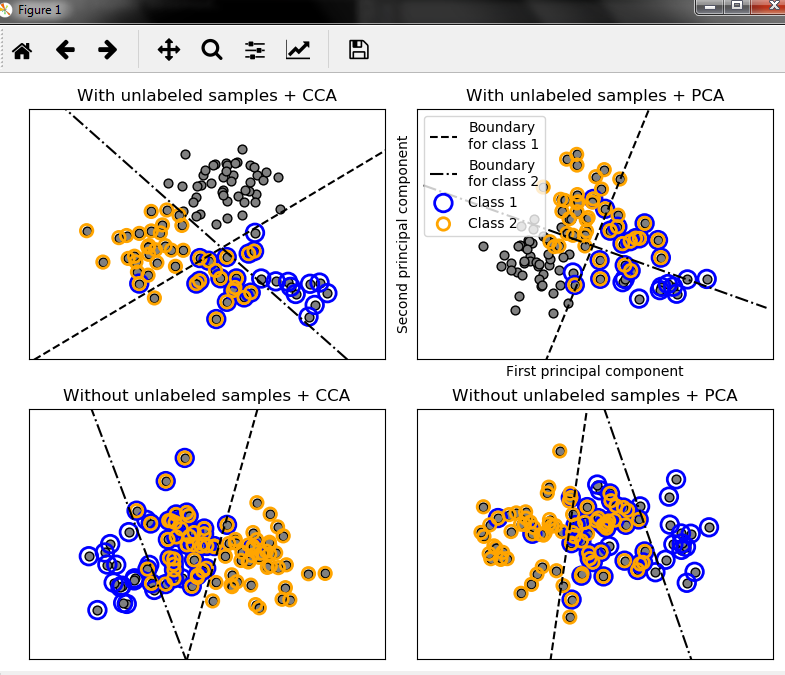
\includegraphics[scale=0.5]{figures/hasil2.png}
   	 \caption{Gambar Yang Muncul Dari Matplotlib}	
	\end{center}
\end{figure}
\end{enumerate}

\subsection{Mencoba Loading an example dataset, menjelaskan maksud dari tulisan tersebut dan mengartikan per baris}

\begin{enumerate}
\item Mengimmport dataset, iris dan digit sebagai contoh data.
\begin{figure}
	\begin{center}
   	 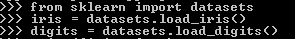
\includegraphics[scale=0.5]{figures/penjelasan1.png}
   	 \caption{Penjelasan }	
	\end{center}
\end{figure}
\item Misalnya, dalam kasus dataset digit, digits.data memberikan akses ke fitur yang dapat digunakan untuk mengklasifikasikan sampel digit.
\begin{figure}
	\begin{center}
   	 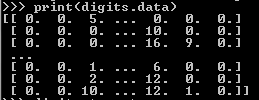
\includegraphics[scale=0.5]{figures/penjelasan2.png}
   	 \caption{Penjelasan 2}	
	\end{center}
\end{figure}
\item Digit.target memberikan kebenaran dasar untuk dataset digit, yaitu angka yang sesuai dengan setiap gambar digit yang dipelajari.
\begin{figure}
	\begin{center}
   	 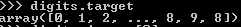
\includegraphics[scale=0.5]{figures/penjelasan3.png}
   	 \caption{Penjelasan 3}	
	\end{center}
\end{figure}
\item Menggambarkan bagaimana mulai dari masalah awal seseorang dapat membentuk data untuk konsumsi di scikit-belajar.
\begin{figure}
	\begin{center}
   	 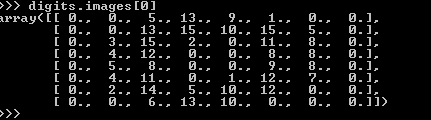
\includegraphics[scale=0.5]{figures/penjelasan4.png}
   	 \caption{Penjelasan 4}	
	\end{center}
\end{figure}

\end{enumerate}

\chapter{Membangun Model Prediksi}
\section{}
\chapter{Prediksi dengan Random Forest}
\section{ TEORI}
\subsection{Random Forest }
\subsubsection{Pengertian}
Random Forest adalah konstruk data yang diterapkan pada machine learning yang mengembangkan sejumlah besar pohon keputusan acak yang menganalisis sekumpulan variabel. Jenis algoritma ini membantu meningkatkan cara teknologi menganalisis data yang kompleks. Juga merupakan algoritma machine learning yang fleksibel, mudah digunakan, bahkan tanpa penyetelan hyper-parameter, dengan hasil yang baik. Ini juga merupakan salah satu algoritma yang paling banyak digunakan, karena kesederhanaan dan faktanya dapat digunakan untuk tugas klasifikasi dan regresi.
Dibawah ini merupakan salah satu ilustrasi penggunaan Random Forest yang saya lakukan untuk memprediksi apakah uang kertas bank otentik atau tidak berdasarkan pada empat atribut.
Ini merupakan hasil dari ilustrasi Random Forest pada Spyder
\begin{figure}[ht]
\centering
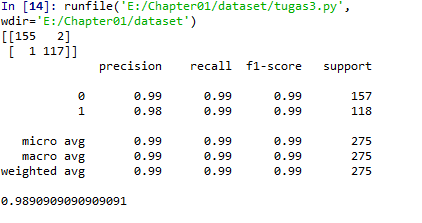
\includegraphics[scale=0.5]{figures/teori1.png}
\caption{Random Forest Spyder}
\label{Contoh}
\end{figure}
\par
Setelah di plotting hasilnya seperti berikut
\begin{figure}[ht]
\centering
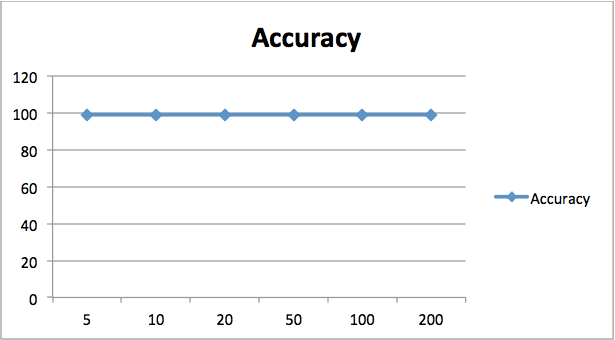
\includegraphics[scale=0.5]{figures/teori2.png}
\caption{Random Forest Graphic}
\label{Contoh}
\end{figure}

\subsection{Dataset}
\subsubsection{Pengertian Dataset}
Dataset adalah kumpulan data. Paling umum satu data set sesuai dengan isi tabel database tunggal, atau matriks data statistik tunggal, di mana setiap kolom tabel mewakili variabel tertentu, dan setiap baris sesuai dengan anggota tertentu dari dataset yang dipertanyakan.
\subsection{Cara Membaca Dataset Dan Arti Setiap File Dan Isi Field Masing Masing File}
\begin{enumerate}
\item
Gunakan librari Pandas pada python untuk dapat membaca dataset dengan format text file.
\item
Setelah itu, buat variabel baru "dataset" yang berisikan perintah untuk membaca file csv. seperti berikut
\begin{figure}[ht]
\centering
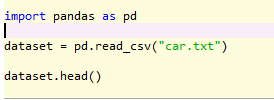
\includegraphics[scale=0.5]{figures/teori3.png}
\caption{Dataset Pandas}
\label{Contoh}
\end{figure}
\par
Pada gambar diatas dapat dijelaskan bahwa :
\begin{itemize}
\item
Memanggil Librari Panda untuk membaca dataset
\item
Membuat variabel "Dataset" yang berisikan pdreadcsv untuk membaca dataset. Pada contoh ini menggunakan txt tapi tetap bisa membaca datasetnya, mengapa? Karena pada saat dijalankan librari panda secara otomatis akan mengubah data dalam bentuk text file ke format csv.
\end{itemize}
\item
Setelah di run akan muncul hasil seperti berikut :
\begin{figure}[ht]
\centering
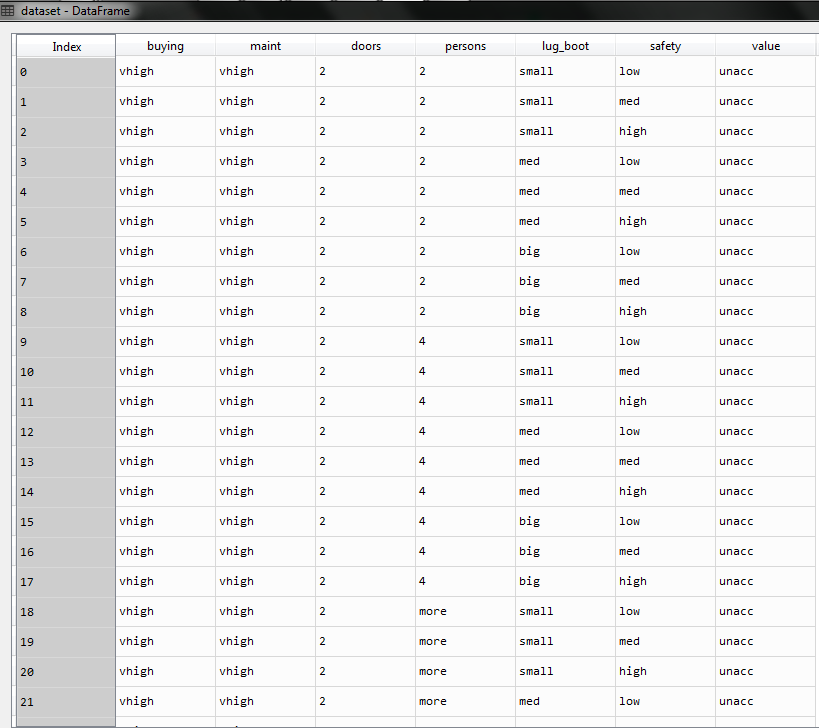
\includegraphics[scale=0.5]{figures/teori4.png}
\caption{Dataset Pandas}
\label{Contoh}
\end{figure}
\par
Pertama tama gambar diatas merupakan dataset yang digunakan untuk evaluasi mobil setelah dibuat untuk mengecek dan menguji induksi konstruktif dan metode penemuan struktur. Datasetnya dapat didapatkan dari laman https://archive.ics.uci.edu/ml/datasets/Car+Evaluation.
Penjelasan dari isi field diatas adalah sebagai berikut :
\begin{itemize}
\item
Atribut Index merupakan atribut otomatis untuk penomoran data yang ada.
\item
Atribut Buying merupakan harga beli dari mobil tersebut. dengan value : v high/Sangat mahal,high/mahal,med/Cukup, low/Murah.
\item
Atribut Maint merupakan harga perawatan dari mobil tersebut, dengan value sama seperti pada atribut Buying.
\item
Atribut Doors merupakan jumlah pintu yang terdapat pada mobil, dengan value 2,3,4,5 more atau lebih dari 5.
\item
Atribut Persons merupakan kapasitas orang yang bisa masuk kedapalm mobil, dengan value 2,4, more /lebih.
\item
Atribut Lug Boot merupakan ukuran bagasi boot mobil, dengan value small,med,big.
\item
Atribut Safety merupakan perkiraan keselamatan mobil, dengan value low,med,high.
\item
Yang terakhir yaitu Value, yang dimana merupakan merupakan Class nya atau disebut dengan targetnya menyatakan apakah mobil tersebut dapat diterima atau tidak dan apakah mobil tersebut bagus atau tidak, dengan value unacc, acc, good,v good .
\end{itemize}
\end{enumerate}

\subsection{Cross Validation}
Cross Validation adalah prosedur resampling yang digunakan untuk mengevaluasi model machine learning pada sampel data yang terbatas. Prosedur ini memiliki parameter tunggal yang disebut k yang mengacu pada jumlah grup tempat sampel data yang akan dibagi. Karena itu, prosedur ini sering disebut k-fold cross-validation.
Proses penentuan apakah hasil numerik yang mengukur hubungan yang dihipotesiskan antar variabel, dapat diterima sebagai deskripsi data, dikenal sebagai Validationi. Umumnya, estimasi kesalahan untuk model dibuat setelah training, lebih dikenal sebagai evaluasi residu. Dalam proses ini, estimasi numerik dari perbedaan respons yang diprediksi dan yang asli dilakukan, juga disebut kesalahan training. Namun, ini hanya memberi kita gambaran tentang seberapa baik model kita pada data yang digunakan untuk melatihnya. Sekarang mungkin bahwa model tersebut kurang cocok atau overfitting data. Jadi, masalah dengan teknik evaluasi ini adalah bahwa itu tidak memberikan indikasi seberapa baik pelajar akan menggeneralisasi ke set data independen / tidak terlihat. Model ini dikenal sebagai Cross Validation.

\subsection{Arti Score 44\% Pada Random Forest, 27\% Pada Decission Tree Dan 29\% Dari SVM}
Itu merupakan presentase keakurasian prediksi yang dilakukan pada saat testing menggunakan label pada dataset yang digunakan. Score merupakan mendefinisikan aturan evaluasi model. Maka pada saat dijalankan akan muncuk persentase tersebut yang menunjukan keakurasian atau keberhasilan dari prediksi yang dilakukan. Jika menggunakan Random Forest maka hasilnya 40\% , jika menggunakan Decission Tree hasil prediksinya yaitu 27\% dan pada SVM 29\% .

\subsection{Confusion Matriks}
\subsubsection{Confusion Matriks Dan Contohnya}
Perthitungan Confusion Matriks dapat dilakukan sebagai berikut. Disini saya menggunakan data yang dibuat sendiri untuk menampilkan data aktual dan prediksi.
\begin{itemize}
\item
Import librari Pandas, Matplotlib, dan Numpy.
\item
Buat variabel y actu yang berisikan data aktual.
\item
Buat variabel y pred berisikan data yang akan dijadikan sebagai prediksi.
\item
Buat variabel df confusion yang berisikan crosstab untuk membangun tabel tabulasi silang yang dapat menunjukkan frekuensi kemunculan kelompok data tertentu.
\item
Pada variabel df confusion definisikan lagi nama baris yaitu Actual dan kolomnya Predicted
\item
Kemudian definisikan suatu fungsi yang diberi nama plot confusion matrix yang berisikan pendefinisian confusion matrix dan juga akan di plotting. untuk code lengkapnya sebagai berikut 
\begin{verbatim}
import numpy as np
import matplotlib.pyplot as plt
import pandas as pd

y_actu = pd.Series([2, 0, 2, 2, 0, 1, 1, 2, 2, 0, 1, 2], name='Actual')
y_pred = pd.Series([0, 0, 2, 1, 0, 2, 1, 0, 2, 0, 2, 2], name='Predicted')
df_confusion = pd.crosstab(y_actu, y_pred)

df_confusion = pd.crosstab(y_actu, y_pred, rownames=['Actual'], colnames=['Predicted'], margins=True)

def plot_confusion_matrix(df_confusion, title='Confusion matrix', cmap=plt.cm.gray_r):
    plt.matshow(df_confusion, cmap=cmap) # imshow
    #plt.title(title)
    plt.colorbar()
    tick_marks = np.arange(len(df_confusion.columns))
    plt.xticks(tick_marks, df_confusion.columns, rotation=45)
    plt.yticks(tick_marks, df_confusion.index)
    #plt.tight_layout()
    plt.ylabel(df_confusion.index.name)
    plt.xlabel(df_confusion.columns.name)

plot_confusion_matrix(df_confusion)

plt.show()
\end{verbatim}

\par

Hasilnya akan seperti berikut :
\begin{figure}[ht]
\centering
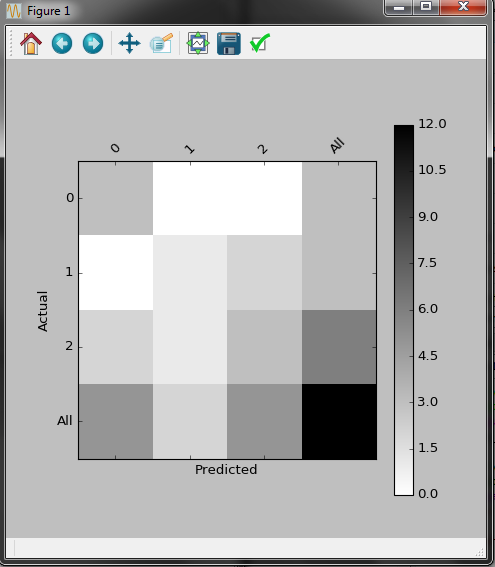
\includegraphics[scale=0.5]{figures/teori5.png}
\caption{Confusion Matrix}
\label{Contoh}
\end{figure}
\end{itemize}

\subsection{Voting Pada Random Forest}
\subsubsection{Pengertian}
Voting yaitu suara untuk setiap target yang diprediksi pada saat melakukan Random Forest. Pertimbangkan target prediksi dengan voting tertinggi sebagai prediksi akhir dari algoritma random forest.
\subsubsection{Contoh}
\begin{itemize}
\item
Untuk menggunakan Voting pada Random Forest dapat dilihat code berikut. Disini saya mengilustrasikan voting untuk berbagai macam algoritma terutama Random Forest.
\begin{verbatim}
import numpy as np
import matplotlib.pyplot as plt

from sklearn.linear_model import LogisticRegression
from sklearn.naive_bayes import GaussianNB
from sklearn.ensemble import RandomForestClassifier
from sklearn.ensemble import VotingClassifier

clf1 = LogisticRegression(solver='lbfgs', max_iter=1000, random_state=123)
clf2 = RandomForestClassifier(n_estimators=100, random_state=123)
clf3 = GaussianNB()
X = np.array([[-1.0, -1.0], [-1.2, -1.4], [-3.4, -2.2], [1.1, 1.2]])
y = np.array([1, 1, 2, 2])

eclf = VotingClassifier(estimators=[('lr', clf1), ('rf', clf2), ('gnb', clf3)],
                        voting='soft',
                        weights=[1, 1, 5])

# predict class probabilities for all classifiers
probas = [c.fit(X, y).predict_proba(X) for c in (clf1, clf2, clf3, eclf)]

# get class probabilities for the first sample in the dataset
class1_1 = [pr[0, 0] for pr in probas]
class2_1 = [pr[0, 1] for pr in probas]


# plotting

N = 4  # number of groups
ind = np.arange(N)  # group positions
width = 0.35  # bar width

fig, ax = plt.subplots()

# bars for classifier 1-3
p1 = ax.bar(ind, np.hstack(([class1_1[:-1], [0]])), width,
            color='green', edgecolor='k')
p2 = ax.bar(ind + width, np.hstack(([class2_1[:-1], [0]])), width,
            color='lightgreen', edgecolor='k')

# bars for VotingClassifier
p3 = ax.bar(ind, [0, 0, 0, class1_1[-1]], width,
            color='blue', edgecolor='k')
p4 = ax.bar(ind + width, [0, 0, 0, class2_1[-1]], width,
            color='steelblue', edgecolor='k')

# plot annotations
plt.axvline(2.8, color='k', linestyle='dashed')
ax.set_xticks(ind + width)
ax.set_xticklabels(['LogisticRegression\nweight 1',
                    'GaussianNB\nweight 1',
                    'RandomForestClassifier\nweight 5',
                    'VotingClassifier\n(average probabilities)'],
                   rotation=40,
                   ha='right')
plt.ylim([0, 1])
plt.title('Class probabilities for sample 1 by different classifiers')
plt.legend([p1[0], p2[0]], ['class 1', 'class 2'], loc='upper left')
plt.tight_layout()
plt.show()
\end{verbatim}
\item
Hasilnya sebagai berikut 
\begin{figure}[ht]
\centering
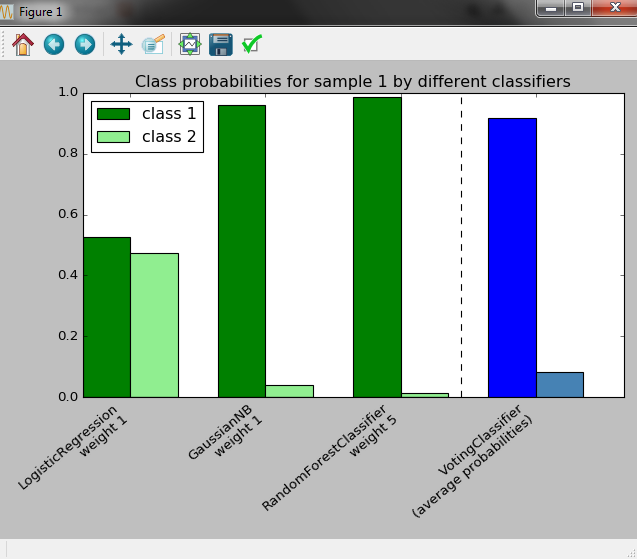
\includegraphics[scale=0.5]{figures/teori6.png}
\caption{Voting Random Forest}
\label{Contoh}
\end{figure}
\end{itemize}


\section{Praktek Program}
\subsection{Aplikasi Sederhana Menggunakan Pandas}
Disini saya akan membuat program sederhana menggunakan Pandas yaitu untuk memilih baris dari DataFrame yang diberikan berdasarkan value di salah satu kolom.
\begin{lstlisting}[caption=Code Program Sederhana Pandas,label={lst:3.1}]
import pandas as pd
d = {'kol1': [1, 4, 3, 4, 5], 'kol2': [4, 5, 6, 7, 8], 'kol3': [7, 8, 9, 0, 1]}
df = pd.DataFrame(data=d)
print("Original DataFrame")
print(df)
print('Baris Untuk kolom2 dengan value 7')
print(df.loc[df['kol2'] == 7 ] )
\end{lstlisting}
Dari code diatas dapat dijelaskan perbarisnya sebagai berikut :
\begin{itemize}
\item
Baris pertama, yaitu import pandas yang artinya kita akan mengimport librari Pandas dari python dengan inisiasi pd.
\item
Variabel d didefinisikan data data untuk kolom 1, kolom2, dan kolom3 
\item
Variabel df akan mengubah data pada variabel d disejajarkan menjadi baris dan kolom dengan menggunakan pd dataframe.
\item
Baris selanjutnya yaitu akan mencetak atau menampilkan tulisan Original dataFrame pada jendela konsol.
\item
Print df artinya akan mencetak atau menampilkan DataFrame dari data yang telah dibuat tadi.
\item
Baris selanjutnya yaitu akan mencetak atau menampilkan tulisan Baris Untuk kolom2 dengan value 7 pada jendela konsol.
\item
Baris terakhir akan menampilkan data yang telah disortir berdasarkan perintah. Dimana hanya akan menampilkan data yang terdapat value 7 pada kolom 2.
\end{itemize}

Hasilnya sebagai berikut :
\begin{figure}[ht]
\centering
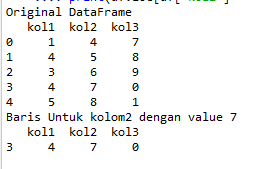
\includegraphics[scale=0.5]{figures/praktek1.png}
\caption{Aplikasi Sederhana Menggunakan Pandas}
\label{Praktek}
\end{figure}

\subsection{ Aplikasi Sederhana Menggunakan Numpy}
Program yang akan dibuat yaitu menentukan atau menemukan  nilai yang sama dari dua array . dapat dilihat dalam lsting \ref{lst:3.2}.
\begin{lstlisting}[caption=Code Program Sederhana Numpy,label={lst:3.2}]
import numpy as np
array1 = np.array([0, 10, 20, 40, 60])
print("Array1: ",array1)
array2 = np.array([10, 30, 40])
print("Array2: ",array2)
print("Data Yang Sama Dari Kedua Array Adalah:")
print(np.intersect1d(array1, array2))
\end{lstlisting}

Dari code diatas dapat dijelaskan perbarisnya sebagai berikut :
\begin{itemize}
\item
Baris pertama, yaitu import numpy yang artinya kita akan mengimport librari Numpy dari python dengan inisiasi np.
\item
Variabel array1 berisikan np array yang dimana akan membuat sebuah Array berisikan value yang telah disebutkan.
\item
Akan mencetak tulisan "Array1" dan menampilkan data dari variabel array1.
\item
Variabel array2 berisikan np array yang dimana akan membuat sebuah Array berisikan value yang telah disebutkan.
\item
Akan mencetak tulisan "Array2" dan menampilkan data dari variabel array2.
\item
Baris selanjutnya akan mencetak dan menampilkan tulisan "Data Yang Sama Dari Kedua Array Adalah:" pada jendela konsol.
\item
Dan yang terakhir np intersect1d akan menampilkan irisan dari array1 dan array2
\end{itemize}

Hasilnya sebagai berikut :
\begin{figure}[ht]
\centering
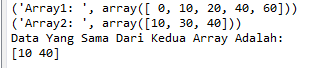
\includegraphics[scale=0.5]{figures/praktek2.png}
\caption{Aplikasi Sederhana Menggunakan Numpy}
\label{Praktek}
\end{figure}
\subsection{Aplikasi Sederhana Menggunakan Matplotlib}
Program yang akan dibuat yaitu membuat dua baris atau lebih dengan lebar dan warna yang berbeda. Code lengkap pada lsting \ref{lst:3.3}
\begin{lstlisting}[caption=Code Program Sederhana Matplotlib,label={lst:3.3}]
import matplotlib.pyplot as plt
# line 1 points
x1 = [10,20,30]
y1 = [20,40,10]
# line 2 points
x2 = [10,20,30]
y2 = [40,10,30]
# Set the x axis label of the current axis.
plt.xlabel('x - Cintaku')
# Set the y axis label of the current axis.
plt.ylabel('y - Cintamu')
# Set a title 
plt.title('Dua Baris Atau Lebih Dengan Lebar Dan Warna Yang Berbeda Guys ')
# Display the figure.
plt.plot(x1,y1, color='salmon', linewidth = 3,  label = 'line1 lebar 3')
plt.plot(x2,y2, color='mediumvioletred', linewidth = 5,  label = 'line2 lebar 5')
# show a legend on the plot
plt.legend()
plt.show()
\end{lstlisting}
Dari code diatas dapat dijelaskan sebagai berikut :
\begin{itemize}
\item
Pertama tama yaitu akan meng import librari Pyplot dari  Matplotlib sebagai plt.
\item
Variabel x1 dan y1 akan berisikan value untuk titik atau point dari garis 1 nya.
\item
Begitu juga dengan variabel x2 dan y2 akan berisikan value untuk titik atau point dari garis 2 nya.
\item
Plt.xlabel akan mengatur label sumbu x dari axis saat ini dengan nama x Cintaku.
\item
Plt.ylabel akan mengatur label sumbu y dari axis saat ini dengan nama x Cintamu.
\item
Plt title akan mendefinisikan title atau judul dari grafik ini.
\item
plt plot akan menampilkan figurenya. Untuk line 1 diberi warna salmon dengan lebar garisnya 3 cm diberi label "line1 lebar 3". Dan untuk  line 2 diberi warna mediumvioletred dengan lebar garisnya 5 cm diberi label "line2 lebar 5".
\item
plt legend untuk menampilkan legend 
\item
Plt show digunakan untuk menampilkan grafik pada saat skrip dijalankan.
\end{itemize}

Hasilnya sebagai berikut :
\begin{figure}[ht]
\centering
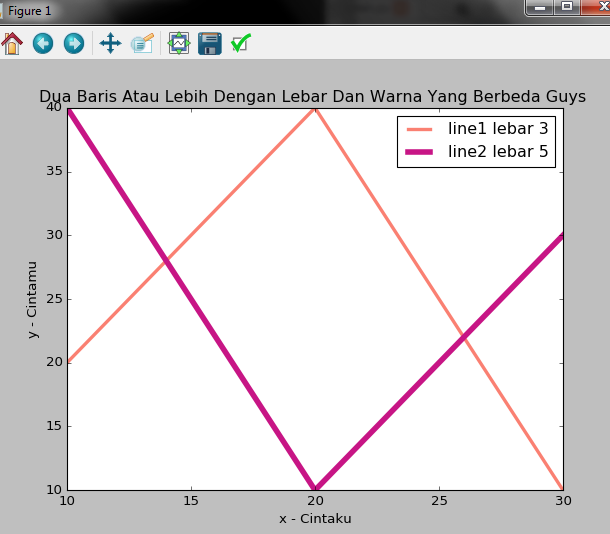
\includegraphics[scale=0.3]{figures/praktek3.png}
\caption{Aplikasi Sederhana Menggunakan Matplotlib}
\label{Praktek}
\end{figure}

\subsection{Menjalankan Program Klasifikasi Random Forest}
Berikut adalah output dari percobaan Random Forest yang telah dilakukan
\begin{itemize}
\item Jika dilihat dari outputnya, code berikut berfungsi untuk membaca data yang berupa dataset dengan format text file. Dengan mendefinisikan variabel imgatt yang berisikan value untuk membaca data, juga menggunakan code untuk skip data yang mengandung bad lines agar tidak terjadi eror pada saat pembacaan file.
\begin{figure}[ht]
\centering
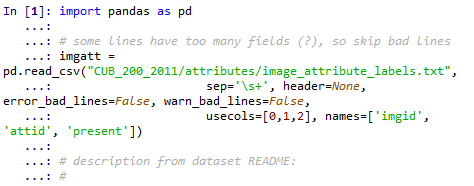
\includegraphics[scale=0.5]{figures/rf1.png}\newpage
\caption{Program Random Forest Tasya}
\label{Praktek}
\end{figure}
\item Output ini mengembalikan baris n teratas (5 secara default) dari dataframe imgatt.
\begin{figure}[ht]
\centering
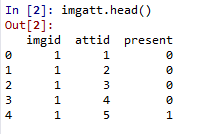
\includegraphics[scale=0.5]{figures/rf2.png}
\caption{Program Random Forest Tasya}
\label{Praktek}
\end{figure}

\item Output ini menampilkan jumlah baris dan kolom dari dataframe imgatt.
\begin{figure}[ht]
\centering
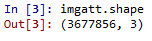
\includegraphics[scale=0.5]{figures/rf3.png}
\caption{Program Random Forest Tasya}
\label{Praktek}
\end{figure}

\item Dari outputnya dapat dilihat bahwa variabel imgatt2 menggunakan function pivot untuk mengubah kolom jadi baris, dan baris jadi kolom dari dataframe sebelumnya.
\begin{figure}[ht]
\centering
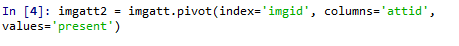
\includegraphics[scale=0.5]{figures/rf4.png}
\caption{Program Random Forest Tasya}
\label{Praktek}
\end{figure}

\item Sama seperti output sebelumnya, imgatt2 head itu berfungsi untuk mengembalikan nilai atau value teratas dari dataframe imgatt2.
\begin{figure}[ht]
\centering
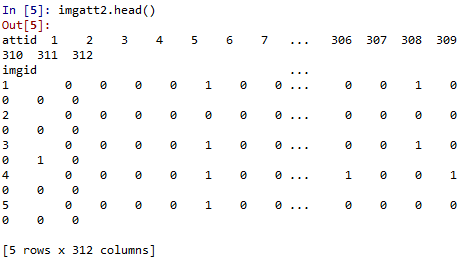
\includegraphics[scale=0.5]{figures/rf5.png}
\caption{Program Random Forest Tasya}
\label{Praktek}
\end{figure}

\item Output ini menampilkan jumlah baris dan kolom dari dataframe imgatt2
\begin{figure}[ht]
\centering
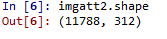
\includegraphics[scale=0.5]{figures/rf6.png}
\caption{Program Random Forest Tasya}
\label{Praktek}
\end{figure}
\item Dan melakukan pivot yang mana imgid menjadi index yang artinya unik.
\begin{figure}[ht]
\centering
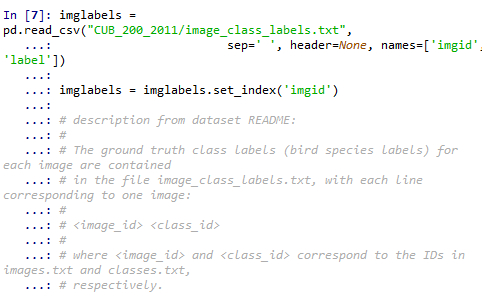
\includegraphics[scale=0.3]{figures/rf7.png}
\caption{Program Random Forest Tasya}
\label{Praktek}
\end{figure}

\item Output diatas akan meload jawabannya yang berisi apakah burung itu termasuk dalam spesies yang mana. Dua kolomnya adalah imgid dan label.
\begin{figure}[ht]
\centering
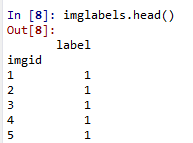
\includegraphics[scale=0.5]{figures/rf8.png}
\caption{Program Random Forest Tasya}
\label{Praktek}
\end{figure}
\item Output dari percobaan sebelumnya, menunjukkan 11788 baris dan 1 kolom. Dimana kolom itu adalah jenis spesies burungnya.
\begin{figure}[ht]
\centering
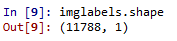
\includegraphics[scale=0.5]{figures/rf9.png}
\caption{Program Random Forest Tasya}
\label{Praktek}
\end{figure}
\item Melakukan join antara imgatt2 dengan imglabels karena isinya sama. Sehingga kita akan mendapatkan data ciri dan data jawabannya atau labelnya sehingga bisa dikatekorikan supervised learning.
\begin{figure}[ht]
\centering
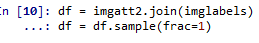
\includegraphics[scale=0.5]{figures/rf10.png}
\caption{Program Random Forest Tasya}
\label{Praktek}
\end{figure}
\item Output diatas akan drop label yang didepan, dan menggunakan label yang paling belakang yang baru di join.
\begin{figure}[ht]
\centering
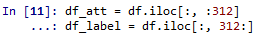
\includegraphics[scale=0.5]{figures/rf11.png}
\caption{Program Random Forest Tasya}
\label{Praktek}
\end{figure}
\item Output berikut mengecek isinya. Ini mengecek 5 data teratas dari df att
\begin{figure}[ht]
\centering
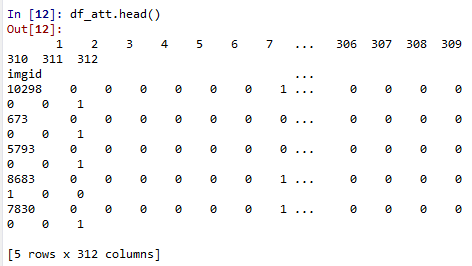
\includegraphics[scale=0.5]{figures/rf12.png}
\caption{Program Random Forest Tasya}
\label{Praktek}
\end{figure}
\item Output berikut mengecek isinya. Ini mengecek 5 data teratas dari df label
\begin{figure}[ht]
\centering
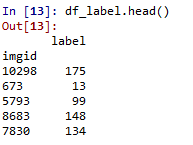
\includegraphics[scale=0.5]{figures/rf13.png}
\caption{Program Random Forest Tasya}
\label{Praktek}
\end{figure}
\item Output diatas membagi menjadi dua bagian, 8000 row pertama sebagai data training sisanya sebagai data testing.
\begin{figure}[ht]
\centering
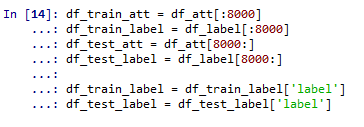
\includegraphics[scale=0.5]{figures/rf14.png}
\caption{Program Random Forest Tasya}
\label{Praktek}
\end{figure}
\item Memanggil kelas RandomForestClassifier. max features diartikan sebagai berapa banyak kolom pada setiap tree disini kolom pada setiap tree adalah 50.
\begin{figure}[ht]
\centering
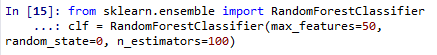
\includegraphics[scale=0.5]{figures/rf15.png}
\caption{Program Random Forest Tasya}
\label{Praktek}
\end{figure}
\item Output ini melakukan fit untuk membangun random forest yang sudah ditentukan dengan maksimum fitur sebanya 50 untuk perpohonnya.
\begin{figure}[ht]
\centering
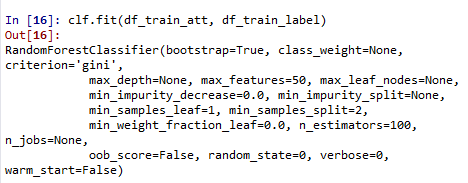
\includegraphics[scale=0.5]{figures/rf16.png}
\caption{Program Random Forest Tasya}
\label{Praktek}
\end{figure}
\item Menampilkan hasil prediksi dari random forest sebelumnya.
\begin{figure}[ht]
\centering
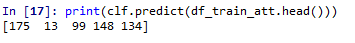
\includegraphics[scale=0.5]{figures/rf17.png}
\caption{Program Random Forest Tasya}
\label{Praktek}
\end{figure}
\item Menampilkan besaran akurasinya dari prediksi diatas atau Score perolehan dari klasifikasi.
\begin{figure}[ht]
\centering
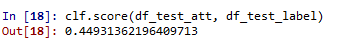
\includegraphics[scale=0.5]{figures/rf18.png}
\caption{Program Random Forest Tasya}
\label{Praktek}
\end{figure}
\end{itemize}

\subsection{Menjalankan Program Confusion Matrix}
Berikut adalah output dari percobaan Confusion Matrix yang telah dilakukan
\begin{itemize}
\item  Memetakan Random Forest ke dalam Confusion Matrix
\begin{figure}[ht]
\centering
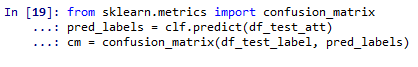
\includegraphics[scale=0.5]{figures/cm1.png}
\caption{Program Confusion Matrix Tasya}
\label{Praktek}
\end{figure} 

\item  Melihat hasil dari gambar diatas
\begin{figure}[ht]
\centering
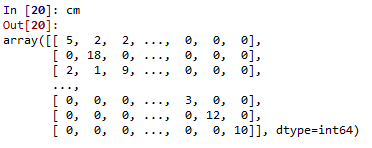
\includegraphics[scale=0.5]{figures/cm2.png}
\caption{Program Confusion Matrix Tasya}
\label{Praktek}
\end{figure} 

\item Plotting Confusion Matrix dengan Matplotlib
\begin{figure}[ht]
\centering
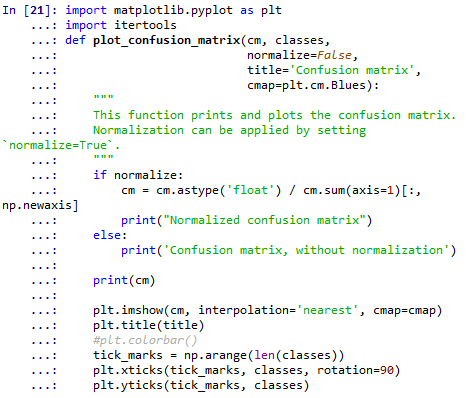
\includegraphics[scale=0.5]{figures/cm3.png}
\caption{Program Confusion Matrix Tasya}
\label{Praktek}
\end{figure}

\item Set plot sumbunya sesuai dengan nama datanya dan membaca file classes txt
\begin{figure}[ht]
\centering
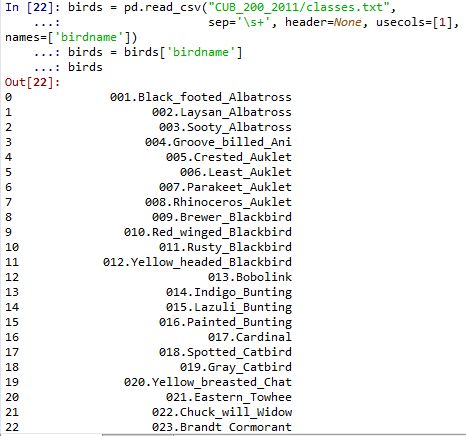
\includegraphics[scale=0.5]{figures/cm4.png}
\caption{Program Confusion Matrix Tasya}
\label{Praktek}
\end{figure}

\item Plot hasil perubahan label
\begin{figure}[ht]
\centering
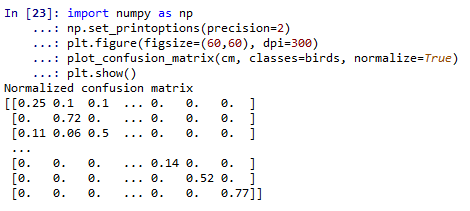
\includegraphics[scale=0.5]{figures/cm5.png}
\caption{Program Confusion Matrix Tasya}
\label{Praktek}
\end{figure}
\end{itemize}

\subsection{Menjalankan Program  Klasifikasi SVM dan Decission Tree}
Berikut adalah output dari percobaan  Klasifikasi SVM dan Decission Tree yang telah dilakukan
\begin{itemize}
\item Mencoba klasifikasi dengan decission tree dengan dataset yang sama dan akan muncul akurasi prediksinya.
\begin{figure}[ht]
\centering
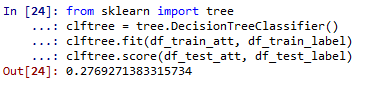
\includegraphics[scale=0.5]{figures/tree1.png}
\caption{Program Decission Tree Tasya}
\label{Praktek}
\end{figure}

\item Mencoba klasifikasi dengan SVM dengan dataset yang sama dan akan muncul akurasi prediksinya.
\begin{figure}[ht]
\centering
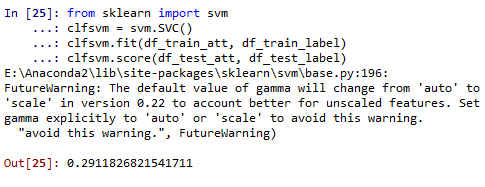
\includegraphics[scale=0.5]{figures/svm1.png}
\caption{Program SVM Tasya}
\label{Praktek}
\end{figure}
\end{itemize}

\subsection{Menjalankan Program Cross Validation}
Berikut adalah output dari percobaan  Cross Validation yang telah dilakukan
\begin{itemize}
\item Hasil Cross Validation untuk  Random Forest
\begin{figure}[ht]
\centering
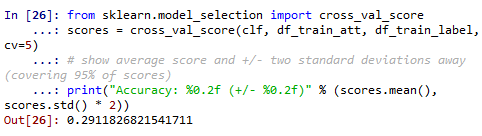
\includegraphics[scale=0.5]{figures/cv1.png}
\caption{Program Cross Validation Tasya}
\label{Praktek}
\end{figure}

\item Hasil Cross Validation untuk Decission Tree
\begin{figure}[ht]
\centering
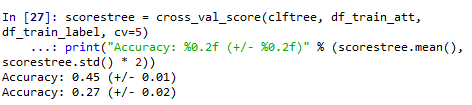
\includegraphics[scale=0.5]{figures/cv2.png}
\caption{Program Cross Validation Tasya}
\label{Praktek}
\end{figure}

\item Hasil Cross Validation untuk SVM
\begin{figure}[ht]
\centering
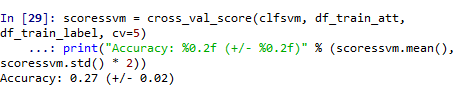
\includegraphics[scale=0.5]{figures/cv3.png}
\caption{Program Cross Validation Tasya}
\label{Praktek}
\end{figure}
\end{itemize}

\subsection{Menjalankan Program Komponen Informasi}
Berikut adalah output dari percobaan Komponen Informasi yang telah dilakukan
\begin{itemize}
\item Dari output ini dapat mengetahui berapa banyak tree yang dibuat, berapa banyak atribut yang dipakai dan informasi lainnya
\begin{figure}[ht]
\centering
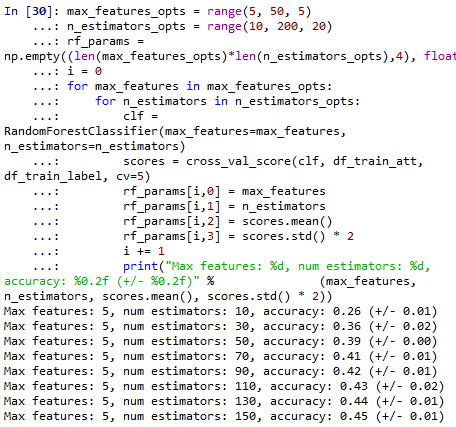
\includegraphics[scale=0.5]{figures/ki1.png}
\caption{Program Komponen Informasi Tasya}
\label{Praktek}
\end{figure}

\item Output berikut merupakan hasil dari plotting komponen informasi agar dapat dibaca
\begin{figure}[ht]
\centering
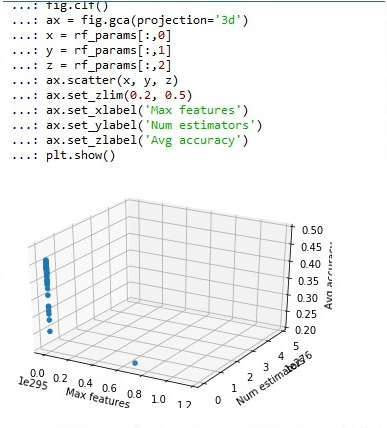
\includegraphics[scale=0.5]{figures/ki2.png}
\caption{Program Komponen Informasi Tasya}
\label{Praktek}
\end{figure}
\end{itemize}

\section{Penanganan Error}
\subsection{Error Index}
\begin{enumerate}
	\item
Berikut ini merupakan eror yang didapatkan saat menjalankan program diatas
\begin{figure}[ht]
\centering
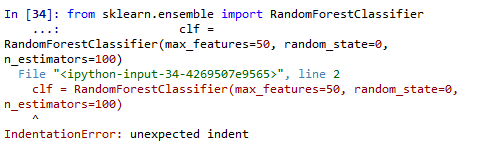
\includegraphics[scale=0.5]{figures/eror3.png}
\caption{Error Index}
\label{Error}
\end{figure}
	\item
Pada gambar diatas kode erornya adalah IndentationError unexpected indent. Eror ini terjadi karena adanya inkosisten pemberian indent di kode program.
	\item
Solusi yang bisa dilakukan untuk mengatasi eror tersebut adalah sebagai berikut : 
\end{enumerate}
\begin{itemize}
\item
Buka file code program dan lihat pada bagian erornya
\begin{figure}[ht]
\centering
\includegraphics[scale=0.5]{figures/solusi9.png}
\caption{File Codingan}
\label{Eror}
\end{figure}
\item
Dapat dilihat pada baris kedua terdapat spasi dibagian depan, hilangkan atau hapus spasi tersebut seperti berikut 
\begin{figure}[ht]
\centering
\includegraphics[scale=0.5]{figures/solusi10.png}
\caption{Menghapus Spasi}
\label{Eror}
\end{figure}
\item Save, kemudian ketika dijalankan eror akan teratasi
\begin{figure}[ht]
\centering
\includegraphics[scale=0.5]{figures/solusi11.png}
\caption{Eror Teratasi}
\label{Eror}
\end{figure}
\end{itemize}

\chapter{Experiment and Result}
\section{Teori}
\subsection{Klasifikasi Teks}
\subsubsection{Pengertian Klasifikasi Teks}
Merupakan salah satu tugas terpenting dalam Pemrosesan Bahasa Alami (Natural Language Processing). Ini adalah proses mengklasifikasikan string teks atau dokumen ke dalam kategori yang berbeda, tergantung pada konten string. Klasifikasi teks memiliki berbagai aplikasi, seperti mendeteksi sentimen pengguna dari tweet, mengklasifikasikan email sebagai spam atau ham, mengklasifikasikan posting blog ke dalam kategori yang berbeda, penandaan otomatis permintaan pelanggan, dan sebagainya. BErikut adalah contoh dari Klasifikasi Teks.
Contohnya, misal kita ingin mencari kata dog, table, on, the . kemudian jika kata yang dimaksud sesuai maka akan menampilkan bilangan biner 1 dan jika salah 0. Seperti dibawah ini :
\begin{figure}[ht]
\centering
\includegraphics[scale=0.5]{figures/chapter4tasya1.png}
\caption{Klasifikasi Teks Tasya}
\label{Contoh}
\end{figure}

\subsection{Klasifikasi Bunga}
Jelaskan mengapa klasifikasi bunga tidak bisa menggunakan machine learning, sertakan ilustrasi sendiri.
Dikarenakan tidak semua bunga memliki ciri - ciri yang sama. Atau dalam kata lain terdapat data noise dalam klasifikasi bunga sehingga tidak bisa menggunakan machine learning.
Contohnya Anggrek memiliki warna ungu, dengan jumlah kelopak 5. Kemudian ada bunga warna ungu dengan jumlah kelopak yang sama namun ternyata bukan anggrek dan kategorinya banyak sekali. Bahkan ada bunga yang tidak jelas apakah warnanya sesuai atau tidak, sehingga bisa menyebabkan data noise.
\begin{figure}[ht]
\centering
\includegraphics[scale=0.5]{figures/chapter4tasya2.png}
\caption{Klasifikasi Bunga Berwana Ungu Tasya}
\label{Contoh}
\end{figure}

\subsection{Pembelajaran Mesin Pada Teks Kata - Kata di Youtube}
Menggunakan teknik bag-of-words pada klasifikasi berbasis text dan kata untuk mengklasifikasikan komentar yang ada di internet sebagai spam atau bukan. Misalkan pada kolom komentar dapat di cek seberapa sering suatu kata muncul dalam kalimat. Setiap kata dapat dijadikan baris dan kolomnya ini merupakan kategori kata terbut, apakah masuk kedalam spam atau tidak. dan contoh lainnya yaitu pada Caption. dimana akan muncul subtitle secara otomatis dari youtube menggunakan sensor suara yang disesuaikan dengan kata yang telah ditentukan. Contohnya seperti berikut :
\begin{figure}[ht]
\centering
\includegraphics[scale=0.5]{figures/chapter4tasya3.png}
\caption{Klasifikasi Comment Spam Di Youtube Tasya}
\label{Contoh}
\end{figure}

\subsection{Arti Score 44\% Pada Random Forest, 27\% Pada Decission Tree Dan 29\% Dari SVM}
Itu merupakan presentase keakurasian prediksi yang dilakukan pada saat testing menggunakan label pada dataset yang digunakan. Score merupakan mendefinisikan aturan evaluasi model. Maka pada saat dijalankan akan muncuk persentase tersebut yang menunjukan keakurasian atau keberhasilan dari prediksi yang dilakukan. Jika menggunakan Random Forest maka hasilnya 40\% , jika menggunakan Decission Tree hasil prediksinya yaitu 27\% dan pada SVM 29\% .

\subsection{Bag of Words}
\subsubsection{Pengertian Bag of Words}
Merupakan representasi teks yang menggambarkan kemunculan kata-kata dalam dokumen. ePngelompokan kata kata kedalam perhitunga, berapakali sebuah kata muncul dalam satu kalimat. Disebut "tas" kata-kata, karena informasi tentang susunan atau struktur kata dalam dokumen dibuang. Model ini hanya berkaitan dengan apakah kata-kata yang diketahui muncul dalam dokumen, bukan di mana dalam dokumen.\\
Contohnya disini akan melihat kemunculan kata dari kalimat :
\begin{enumerate}
\item I Love Dogs
\item I hate dogs and knitting
\item Knitting is my hobby and passion.
\end{enumerate}
\begin{figure}[ht]
\centering
\includegraphics[scale=0.5]{figures/chapter4tasya4.png}
\caption{Bag of Words Tasya}
\label{Contoh}
\end{figure}

\subsection{TF-IDF}
TF-IDF  memberi kita frekuensi kata dalam setiap dokumen dalam korpus atau mengganti data jadi number. Ini adalah rasio berapa kali kata itu muncul dalam dokumen dibandingkan dengan jumlah total kata dalam dokumen itu. Itu meningkat seiring jumlah kemunculan kata itu di dalam dokumen meningkat. Setiap dokumen memiliki tf sendiri. Dalam ilustrasi disini saya akan mengganti contoh Bag of Words menjadi bentuk TF-IDF.
\begin{figure}[ht]
\centering
\includegraphics[scale=0.5]{figures/chapter4tasya5.png}
\caption{Contoh TF-IDF Tasya}
\label{Contoh}
\end{figure}

\section{PRAKTIKUM}
\subsection{Aplikasi Sederhana Menggunakan Pandas}
Disini saya akan menggunakana Dataset dari https://www.kaggle.com/spscientist/students-performance-in-exams dan akan mengambil Data Dummy sebanyak 500 records dan membuat Dataframe baru.
\begin{verbatim}
import pandas as pd
mhs = pd.read_csv('StudentsPerformanceExam.csv', sep=';')
df = pd.DataFrame(mhs, columns = ['gender', 'race/ethnicity', 'parental level of education', 'lunch', 'test preparation course', 'math score', 'reading score', 'writing score'])

dummy = pd.get_dummies (df['test preparation course'])
dummy.head()

df = df.join(dummy)
\end{verbatim}
Maksud dari kodingan diatas yaitu :
\begin{enumerate}
\item Baris pertama impor librari pandas dengan inisiasi pd
\item Definisikan variabel mhs untuk membaca file csv dengan pandas
\item variabel df akan menggunakan function pddataframe untuk membuat datafarme di pandas dari file CSV yang tadi.
\item Mendefinisikan variabel dummy untuk mengubah data categorical menjadi integer. dibahwa merupakan data sebelum di Dummy.
\begin{figure}[ht]
\centering
\includegraphics[scale=0.5]{figures/praktektasya2.png}
\caption{Dataset Original Tasya}
\label{Aplikasi Pandas}
\end{figure}

\item Atribut atau kolom yang ingin di Dummy yaitu test preparation course. Dalam test preparation course terdapat dua value yaitu Completed dan none. Yang jika di dummy maka valuenya akan berubah menjadi 1 dan 0 seperti berikut :
\begin{figure}[ht]
\centering
\includegraphics[scale=0.5]{figures/praktektasya3.png}
\caption{Dataset Dummy Tasya}
\label{Aplikasi Pandas}
\end{figure}
\item kemudian df akan melakukan join dengan dataframe dummy.
\end{enumerate}

\subsection{Memecah DataFrame Menjadi 2 Dataframe}
Dari dataframe tersebut dipecah menjadi dua dataframe yaitu 450 row pertama dan 50 row sisanya
\begin{verbatim}
mhs_train= mhs[:450]
mhs_test= mhs[451:]
\end{verbatim}
\begin{enumerate}
\item mhs train akan mendefinisikan dataframe untuk train dengan 450 data pertama
\item mhs test mendefinisikan dataframe untuk test untuk data setelah 451. Hasilnya seperti berikut :
\end{enumerate}
\begin{figure}[ht]
\centering
\includegraphics[scale=0.5]{figures/praktektasya4.png}
\caption{Split DataFrame Tasya}
\label{Aplikasi Pandas}
\end{figure}

\subsection{ Vektorisasi Dan Klasifikasi Dari Data Youtube Eminem Dengan Decision Tree}
\begin{enumerate}
\item Ini hasil dari impor dataset
\begin{figure}[ht]
\centering
\includegraphics[scale=0.5]{figures/praktektasya7.png}
\caption{Dataset Youtube Eminem Tasya}
\label{Praktek}
\end{figure}
\item Ini hasil Setelah di Klasifikasikan dengan Decision Tree
\begin{figure}[ht]
\centering
\includegraphics[scale=0.5]{figures/praktektasya6.png}
\caption{Dataset Youtube Eminem Tasya}
\label{Praktek}
\end{figure}
\item Dalam in 52 impor Tree dari Sklearn. Dan mendefinisikan variabel clf untuk memanggil Decision Tree Classifier dan melakukan fit atau pengujian
\item Dalam In 53 menggunakan prediksi untuk clf dengan function predict  untuk memprediksi test. Dan hasilnya muncul dalam bentuk array.
\item clf score memunculkan akurasi prediksi yang dilakukan terhadap clf.
\end{enumerate}

\subsection{Vektorisasi Dan Klasifikasi Dari Data Youtube Eminem Dengan SVM}
\begin{figure}[ht]
\centering
\includegraphics[scale=0.5]{figures/praktektasya8.png}
\caption{Dataset Youtube Eminem SVM Tasya}
\label{Praktek}
\end{figure}
Dari Gambar diatas dapat dijelaskan bahwa :
\begin{enumerate}
\item Impor SVM dari sklearn
\item Melakukan fit dari d train att dan d train label atau disebut dengan pengujian
\item Mendefinisikan variabel clf untuk melakukan prediksi dataset Youtube Eminem dengan SVM. Dan akan muncul hasil prediksinya
\end{enumerate}

\subsection{Vektorisasi Dan Klasifikasi Dari Data Youtube Eminem Dengan Decision Tree 2}
\begin{figure}[ht]
\centering
\includegraphics[scale=0.5]{figures/praktektasya9.png}
\caption{Dataset Youtube Eminem Tasya}
\label{Praktek}
\end{figure}
Maksud dari codingan diatas yaitu, mengkasifikasikan Dataset Youtube Eminem dengan Decision Tree dengan melakukan prediksi menggunakan function test pada d test att, dan memberikan akurasi prediksi menggunakan prediksi score.

\subsection{Plotting Confusion Matrix}
Berikut adalah skripl dari plotting confusion matrix dari contoh yang ada pada bagian teori
\begin{verbatim}
import matplotlib.pyplot as plt
import itertools
def plot_confusion_matrix(cm, classes,
                          normalize=False,
                          title='Confusion matrix',
                          cmap=plt.cm.Blues):
    """
    This function prints and plots the confusion matrix.
    Normalization can be applied by setting `normalize=True`.
    """
    if normalize:
        cm = cm.astype('float') / cm.sum(axis=1)[:, np.newaxis]
        print("Normalized confusion matrix")
    else:
        print('Confusion matrix, without normalization')

    print(cm)

    plt.imshow(cm, interpolation='nearest', cmap=cmap)
    plt.title(title)
    #plt.colorbar()
    tick_marks = np.arange(len(classes))
    plt.xticks(tick_marks, classes, rotation=90)
    plt.yticks(tick_marks, classes)

    fmt = '.2f' if normalize else 'd'
    thresh = cm.max() / 2.
    #for i, j in itertools.product(range(cm.shape[0]), range(cm.shape[1])):
    #    plt.text(j, i, format(cm[i, j], fmt),
    #             horizontalalignment="center",
    #             color="white" if cm[i, j] > thresh else "black")

    plt.tight_layout()
    plt.ylabel('True label')
    plt.xlabel('Predicted label')


import numpy as np
np.set_printoptions(precision=2)
plt.figure(figsize=(60,60), dpi=300)
plot_confusion_matrix(cm, classes=clf, normalize=True)
plt.show()
\end{verbatim}
Hasilnya adalah sebagai berikut :
\begin{figure}[ht]
\centering
\includegraphics[scale=0.5]{figures/praktektasya10.png}
\caption{Confusion Matrix Tasya}
\label{Praktek}
\end{figure}
Dari gambar dapat dijelaskan bahwa data array merupakan data asli dan data prediksi yang dilakukan dengan Random Forest. DEngan melakukan normalisasi data confusion matrix.

\subsection{ Menjalankan Program Cross Validation}
\begin{figure}[ht]
\centering
\includegraphics[scale=0.5]{figures/praktektasya5.png}
\caption{Cross Validation Tasya}
\label{Aplikasi Pandas}
\end{figure}
Gambar diatas akan dijelaskan seperti berikut :
\begin{enumerate}
\item Dari sklearn mengimpor Cross Validation
\item Variabel scores akan melakukan cross validation pada variabel clf, d train att , dan d train label
\item Variabel skorrata2 akan menghitung nilai rata rata dari variabel scores tadi menggunakan function mean
\item skoresd Menghitung standar deviasi dari data yang diberikan. Hssilnya seperti berikut :
\end{enumerate}
\begin{figure}[ht]
\centering
\includegraphics[scale=0.5]{figures/praktektasya6.png}
\caption{Hasil Cross Validation Tasya}
\label{Cross Validation}
\end{figure}

\subsection{Program Pengamatan Komponen Informasi}
\begin{figure}[ht]
\centering
\includegraphics[scale=0.5]{figures/praktektasya11.png}
\caption{Program Komponen Informas Tasyai}
\label{Praktek}
\end{figure}
Dari gambar diatas dapat dijelaskan bahwa :
\begin{enumerate}
\item Max featuresnya dari range 5 sampai 50
\item n estimators dengan range 10 sampai 150
\item Variabel rf params berisikan function np empty dimana akan membuat array baru berisikan tipe yang didefinisikan dengan random value
\item Mendefinisika i dimulai dari angka 0 dimana max features dan n estimators menggunakan klasifikasi randomforestclassifier menggunakan data prediksi
\item Mendefinisikan rfparams untuk max features , n estimators, nilai rata dan std
\end{enumerate}

\section{Penanganan Error}
\subsection{Error Index}
\begin{enumerate}
	\item
Berikut ini merupakan eror yang didapatkan saat menjalankan program diatas
\begin{figure}[ht]
\centering
\includegraphics[scale=0.5]{figures/praktektasyaeror1.png}
\caption{Error Key Tasya }
\label{Error}
\end{figure}
\item
Pada gambar diatas kode erornya adalah KeyEror. Eror ini terjadi karena keyword yang dimasukan tidak ada.
\item
Solusi yang bisa dilakukan untuk mengatasi eror tersebut adalah sebagai berikut :
\end{enumerate}
\begin{itemize}
\item
\begin{figure}[ht]
\centering
\includegraphics[scale=0.5]{figures/praktektasyaeror2.png}
\caption{Error Key Tasya}
\label{Error}
\end{figure}
Pada gambar diatas Dataset StudentPerformanceExam tidak terdapat atribut student, maka dari itu kita harus merubahnya dengan atribut yang terdapat di dataset tersebut. Mari kita gunakan atribut gender. Ubah skrip menjadi seperti berikut
\item
\begin{figure}[ht]
\centering
\includegraphics[scale=0.5]{figures/praktektasyaeror3.png}
\caption{Error Key Tasya}
\label{Error}
\end{figure}
\item Maka ketika di run akan muncul data dummy nya seperti berikut
\begin{figure}[ht]
\centering
\includegraphics[scale=0.5]{figures/praktektasyaeror4.png}
\caption{Error Key Tasya}
\label{Error}
\end{figure}
\end{itemize}


\chapter{Vektorisasi Kata dan Dokumen}

\section{Teori}
\subsection{Vektorisasi}
Karena ketika menggunakan algoritma machine learning tidak bisa  secara langsung menggunakan teks melainkan teks tersebut harus diubah menjadi angka. Kita membutuhkan cara untuk merepresentasikan data teks untuk algoritma pembelajaran mesin, vektorirasi membantu mengubah teks biasa kedalam bentuk vektor yang dapat dimengerti oleh komputer atau machine learning. Kita mungkin ingin melakukan klasifikasi dokumen, sehingga setiap dokumen adalah "input" dan label kelas adalah "output" untuk algoritma prediksinyai. Algoritma mengambil vektor angka sebagai input, oleh karena itu kita perlu mengkonversi dokumen menjadi vektor angka dengan panjang tetap atau sama.
\par Untuk ilustrasinya misal,  saya memiliki kamus berisikan kata-kata {MonkeyLearn, is, not, great}, dan saya ingin membuat vektor teks "MonkeyLearn is great", saya akan memiliki vektor berikut: (1, 1, 0, 0, 1,) .

\subsection{Vektor Dataset Google}
Karena di dalam satu dataset berisikan setidaknya 3 Milyar kata dan kalimat. Yang dimana dimensi berisikan kata - kata unik dari data tersebut. Maka dari itu dimensi pada dataset Google bisa mencapai 300.

Untuk ilustrasinya, misalkan kita memiliki sebuah buku dengan tebal 1000 , dimana bukunya dibagi menjadi dua Chapter. Kemudian kita akan menggabungkan kata dari setiap Chapter tersebut. Maka akan didapatkan irisan yang akan berjumlah lebih dari 200. dikarenakan banyak kata yang berbeda beda.

\subsection{Konsep Vektorisasi Untuk Kata}
Konsepnya yaitu kata atau teks akan dihapuskan noisy datanya atau dihapus data yang tidak terpakai, seperti tag html jika ada, titik, koma, dll. Kemudian tokenization artinya kita akan mengelompokan kalimat menjadi token atua membagi kata kata menjadi potingan kecil. Baru setelah itu dilakukan normalisasi untuk mengubah datanya menjadi angka.

Ilustrasinya, misalnya ada beberapa kalimat seperti berikut :
\begin{itemize}
\item There used to be Iron Age.

Kemudian didapatkan token seperti berikut “There”,”was”,”to”,”be”,”used”,”Stone”,”Bronze,”Iron”,”Revolution”,”Digital”,”Age”,”of”,”Now”,”it”,”is”

Maka ketika di cek pada kalimat diatas hasilya seperti berikut 
\item There used to be iron age = [1,0,1,1,1,0,0,1,0,0,1,0,0,0,0]
\end{itemize}

\subsection{Konsep Vektorisasi Untuk Dokumen}
Hampir mirip dengan konsep kata, namun untuk di dokumen biasanya konsepnya digunakan untuk mencari kesamaan atau memprediksi seberapa sering menculan kata dalam 2 kalimat atau 2 paragraf.

Ilustrasinya, misalkan dalam sebuah artikel kita ingin mencari seberapa banyak kata "dimana" muncul. Maka dengan Doc2Vec dapat diprediksi hasilnya.

\subsection{Mean Dan Standar Deviasi}
\subsubsection{Pengertian}
Mean adalah nilai rata-rata dari beberapa buah data. Nilai mean dapat ditentukan dengan membagi jumlah data dengan banyaknya data.

Deviasi standar adalah ukuran ringkasan perbedaan setiap pengamatan dari rata-rata. Deviasi standar mengukur penyebaran data tentang nilai rata-rata. Ini berguna dalam membandingkan set data yang mungkin memiliki mean yang sama tetapi rentang yang berbeda.

\subsubsection{Contoh}
\begin{enumerate}
\item Misalkan kita sudah menghitung tinggi anjing.
\begin{figure}[ht]
\centering
\includegraphics[scale=0.5]{figures/chapter5tasya1.png}
\caption{Contoh Mean dan Standar Deviasi }
\label{Teori}
\end{figure}
\item Tingginya dilihat dari bahu : 600mm, 470mm, 170mm, 430mm and 300mm.
\item Kita hitung mean atau rata ratanya, dengan menjumlahkan seluruh data dan membaginya dengan jumlah n nya hasilnya yaitu 394.
\item Kemudian kita ingin melihat berapa perbedaan tinggi dari anjing - anjing tersebut menggunakan variance. 
\item Baru Gunakan standar deviasi didapatkan hasil 147 mm . DEngan Deviasi Standar kita bisa tahau mana anjing dengan tinggi normal dan anjing yang kekurangan tinggi.
\begin{figure}[ht]
\centering
\includegraphics[scale=0.5]{figures/chapter5tasya2.png}
\caption{Contoh Mean dan Standar Deviasi }
\label{Teori}
\end{figure}

\subsection{Skip-gram}
Arsitektur model Skip-gram biasanya  mencoba untuk memprediksi kata konteks sumber (kata-kata sekitarnya) diberi kata target (kata tengah). Contohnya seperti berikut 
\begin{figure}[ht]
\centering
\includegraphics[scale=0.5]{figures/chapter5tasya3.png}
\caption{Contoh Skipgram }
\label{Teori}
\end{figure}
\end{enumerate}



\section{PRAKTEK PROGRAM}
\subsection{Mencoba Dataset}
\subsubsection{Vektor}
\begin{itemize}
\item Pada gambar diatas dapat dilihat bahwa vektor memiliki array sebanyak 300 dimensi. Untuk identitas sektor satu adalah 0.10
\begin{figure}[ht]
\centering
\includegraphics[scale=0.5]{figures/chapter5tasya4.png}
\caption{Vektor Love Tasya}
\label{Praktek}
\end{figure}


\item Pada gambar diatas untuk vektor faith dapat dilihat memliki nilai 0.26 , untuk similaritasnya cukup mendekati vektor love dimana faith dapat dikategorikan dalam satu kategori dengan love.
\begin{figure}[ht]
\centering
\includegraphics[scale=0.5]{figures/chapter5tasya5.png}
\caption{Vektor Faith Tasya}
\label{Praktek}
\end{figure}


\item Vektor fall hanya memiliki nilai minus yaitu -0.04 , dimana mesin memahami bahwa fall tidak terdapat dalam satu kategori yang sama dengan love dan faith
\begin{figure}[ht]
\centering
\includegraphics[scale=0.5]{figures/chapter5tasya6.png}
\caption{Vektor Fall Tasya}
\label{Praktek}
\end{figure}


\item  Vektor sick memiliki nilai identitas 1.82 dimana tidak mendekati love, faith maupun fall.
\begin{figure}[ht]
\centering
\includegraphics[scale=0.5]{figures/chapter5tasya7.png}
\caption{Vektor Sick Tasya}
\label{Praktek}
\end{figure}


\item Vektor clear memiliki nilai identitas -2,44 dan tidak mendekati nilai dari vektor fall sehingga tidak dapat dijadikan dalam satu kategori
\begin{figure}[ht]
\centering
\includegraphics[scale=0.3]{figures/chapter5tasya8.png}
\caption{Vektor Clear Tasya}
\label{Praktek}
\end{figure}

\item Untuk vektor shine -0.12 tidak mendekati vektor manapun.
\begin{figure}[ht]
\centering
\includegraphics[scale=0.3]{figures/chapter5tasya9.png}
\caption{Vektor Shine Tasya}
\label{Praktek}
\end{figure}


\item Vektor bag memiliki i=nilai identitas -0.03 yang mendekati dengan vektor fall. SEhingga mesin memahami bahwa mungkin saja kedua vektor tersebut berada dalam satu kategori.
\begin{figure}[ht]
\centering
\includegraphics[scale=0.3]{figures/chapter5tasya10.png}
\caption{Vektor Bag Tasya}
\label{Praktek}
\end{figure}


\item Vektor car nilainya 0.13 mendekati vektor love dan faith sehingga mungkin dapat dikategorikan dalam satu kategori.
\begin{figure}[ht]
\centering
\includegraphics[scale=0.3]{figures/chapter5tasya11.png}
\caption{Vektor Car Tasya}
\label{Praktek}
\end{figure}


\item Vektor wash memiliki nilai 9.46 jauh dari vektor vektor lainnya.
\begin{figure}[ht]
\centering
\includegraphics[scale=0.3]{figures/chapter5tasya12.png}
\caption{Vektor Wash Tasya}
\label{Praktek}
\end{figure}


\item Vektor motor memiliki nilai identitas 5.73 yang bisa mendekati vektor wash. Dapat dikatakan bahwa motor dapat dicuci jika diarti dalam satu kategori yang sama.
\begin{figure}[ht]
\centering
\includegraphics[scale=0.3]{figures/chapter5tasya13.png}
\caption{Vektor Motor Tasya}
\label{Praktek}
\end{figure}
\end{itemize}

\subsubsection{Similariti}
\begin{enumerate}
\item Lihat gambar berikut yang merupakan hasil prediksi similariti
\begin{figure}[ht]
\centering
\includegraphics[scale=0.3]{figures/chapter5tasya17.png}
\caption{Similariti Tasya}
\label{Praktek}
\end{figure}

Dapat disimpulkan bahwa
\begin{itemize}
\item Untuk Love dan faith hasilnya adalah 37%
\item Untuk Love dan fall hasilnya adalah 11%
\item Untuk Love dan sick hasilnya adalah 26%
\item Untuk Love dan clear hasilnya adalah 6%
\item Untuk Love dan shine hasilnya adalah 20%
\item Artinya love dan faith memang dalam kategoruiyang sama misalnya dalam kategori percintaan. MEsin sudah mengetahui bahwa keduanya dapat dikategorikan sebagai percintaan.
\end{itemize}
\end{enumerate}

\subsection{Extract Words dan PermuteSentences}
\subsubsection{Extract Words}
ExtractWords merupakan function untuk menambahkan, menghilangkan atau menghapuskan, hal hal yang tidak penting atau tidakperlu di dalam teks. Dalam contoh dibawah ini. menggunakan function extract words untuk menghapus komen dengan python style , mencari data yang diinginkan, dan memberikan spasi pada teks.
\begin{figure}[ht]
\centering
\includegraphics[scale=0.3]{figures/chapter5tasya15.png}
\caption{Extract Words Tasya}
\label{Praktek}
\end{figure}

\subsubsection{PermuteSentences}
PermuteSentences merupakan class yang digunakan unutm melakukan pengocokan secara acak pada data yang ada. Digunakan cara ini agar tidak terjadi kelebihan memori pada saat dijalankan. Contoh dibawah yaitu fungsi akan memanggil lenght. Yang kemudian mendefinisikan variabel req untuk lenght dam melakukan random choice yaitu pengocokan acak untuk kata car.
\begin{figure}[ht]
\centering
\includegraphics[scale=0.3]{figures/chapter5tasya16.png}
\caption{PermuteSentencesi Tasya}
\label{Praktek}
\end{figure}

\subsection{Fungsi Librari gensim TaggedDocument dan Doc2Vec}
Doc2vec adalah algoritma unsupervised untuk menghasilkan vektor untuk kalimat / paragraf / dokumen. Dan TaggedDocument merupaka function dari Doc2Vec untuk menampilkan tag kata atau kalimat yang diinginkan dari sebuah dokumen.

\begin{itemize}
\item Impor modul TaggedDocument dan modul Doc2Vec
\item Hasilnya seperti berikut
\begin{figure}[ht]
\centering
\includegraphics[scale=0.5]{figures/chapter5tasya18.png}
\caption{TaggedDocument Tasya }
\label{Praktek}
\end{figure}
\end{itemize}


\subsection{Menambahkan data Training Dari File Dengan Doc2Vec}
Yang harus dilakukan yaitu :
\begin{enumerate}
\item Import librari re atau request dari python dan import modul os untuk memungkinkan kita menggunakan operasi sistem sesuai yang dibutuhkan.
\item Medefinisikan variabel unsup sentences yang berisikan variabel kosong.
\item Panggil data training dan data testing dari file yang telah disediakan
\item Kemudian coba data tersebut
\end{enumerate}

Untuk lebih jelasnya, berikut hasil percobaan dari praktek yang dilakukan
\begin{verbatim}
for dirname in ["/train/pos", "/train/neg", "/train/unsup", "/test/pos", "/test/neg"]:
    for fname in sorted (os.listdir("aclImdb/"+dirname)):
        if fname[-4:] == '.txt':
            with open("aclImdb/"+dirname+"/"+ fname, encoding = 'UTF-8') as f:
                sent = f.read()
                words = extract_words(sent)
                unsup_sentences.append(TaggedDocument(words,[dirname+"/"+fname]))
\end{verbatim}
\begin{itemize}
\item Untuk skrip diatas mengambil contoh dataset dari Imdb yang kemudian memanggil data training dan data testing nya.
\item File tersebut diambil dari folder aclImdb
\item File yang dibuka berbentuk teks atau berekstensi txt
\item Kemudian file yang dibuka tadi diasiasikan sebagai f
\item variabel sent akan membaca f
\item Variabel words akan memanggil dan mengirimkan fungsi extract words dari skrip sebelumnya
\item KEmudian list dari unsup sentences akan diupdate dengan menambahkan objek baru dan diberi tag. berikut hasilnya
\begin{figure}[ht]
\centering
\includegraphics[scale=0.5]{figures/chapter5tasya20.png}
\caption{Data Training Imdb Tasya}
\label{Praktek}
\end{figure}
\end{itemize}
\begin{itemize}
\item Untuk contoh dibawah pun sama seperti ynag diatas, bedanya hanya untuk contoh kedua ini dilakukan proses token dan datasetnya dari review polarity.
\begin{figure}[ht]
\centering
\includegraphics[scale=0.5]{figures/chapter5tasya21.png}
\caption{Data Training Polarity Tasya}
\label{Praktek}
\end{figure}

\item Untuk contoh dibawah pun sama seperti yang diatas, bedanya hanya untuk contoh kedua ini dilakukan proses token dan datasetnya dari review rotten tomatoes.
\begin{figure}[ht]
\centering
\includegraphics[scale=0.5]{figures/chapter5tasya22.jpg}
\caption{Data Training Tomatoes}
\label{Praktek}
\end{figure}
\end{itemize}

\subsection{Mengapa Harus Dilakukan Pengocokan Dan Pembersihan Data}
Pengocokan dilakukan untuk mendapatkan hasil yang lebih akurat pada saat melakukan score, karena pengocokan mempengaruhi performa positif negatifnya dari scoring.

Kemudian Pembersihan data dilakukan untuk membersihkan tag spasi ataupun data noisy yang tidak diperlukan dalam dokumen.
\begin{itemize}
\item Import dulu librari re atau request
\item Kemudian Disini akan mendefinisikan function extract words untuk menghapus tag html, hapus tanda petik dan lainnya
\item Setelah itu Data akan dirandomatau dilakukan pengocokan dengan mengimport librari modul dengan mendefinisikan class PermuteSentences. BErikut skrip lengkapnya
\item \begin{verbatim}
import re
def extract_words(sent):
    sent = sent.lower()
    sent = re.sub(r'<[^>]+>', ' ', sent) #hapus tag html
    sent = re.sub(r'(\w)\'(\w)', ' ', sent) #hapus petik satu
    sent = re.sub(r'\W', ' ', sent) #hapus tanda baca
    sent = re.sub(r'\s+', ' ', sent) #hapus spasi yang berurutan
    return sent.split()

import random
class PermuteSentences(object):
    def __init__(self, sents):
        self.sents=sents
        
    def __iter__(self):
        shuffled = list(self.sents)
        random.shuffle(shuffled)
        for sent in shuffled:
            yield sent
\end{verbatim}
\item Berikut merupakan hasil dari pengocokan dan pembersihan data
\begin{figure}[ht]
\centering
\includegraphics[scale=0.5]{figures/chapter5tasya19.png}
\caption{Pengcokan Dan Pembersihan Data Tasya}
\label{Praktek}
\end{figure}
\end{itemize}

\subsection{Mengapa Model Harus Di Save Dan Temporari Training Harus Dihapus}
\begin{itemize}
\item Sebelum model di save atau disipman lakukan pengocokan terlebih dahulu seperti berikut.
\begin{figure}[ht]
\centering
\includegraphics[scale=0.5]{figures/chapter5tasya23.jpg}
\caption{Save Model Tasya}
\label{Praktek}
\end{figure}
\item Kemudian setelah itu gunakan perintah Doc2Vec load dan memasukan nama file setelah disimpan.
\begin{figure}[ht]
\centering
\includegraphics[scale=0.5]{figures/chapter5tasya24.jpg}
\caption{Save Model Tasya}
\label{Praktek}
\end{figure}
\item Ketika model telah di save, barulah hapus temporari dengan skrip berikut. Maka hasil dari kedua praktek diatas adalah sebagi berikut
\begin{figure}[ht]
\centering
\includegraphics[scale=0.5]{figures/chapter5tasya25.jpg}
\caption{Save Model HAsil Tasya}
\label{Praktek}
\end{figure}
\begin{figure}[ht]
\centering
\includegraphics[scale=0.5]{figures/chapter5tasya26.jpg}
\caption{Save Model  HasilTasya}
\label{Praktek}
\end{figure}

Hal yang dapat disimpulkan yaitu :
Model disave untuk memudahkan kita dalam meng-edit file, kita tidak perlu mengetik ulang semua skrip dan tinggal membuka file tersebut jika ingin menguji ulang modelnya.
Temporari training merupakan data training yang sebelumnya kita gunakan untuk mencoba skripnya, namun karena kita telah membuat modelnya dan untuk menghemat memori dilakukan penghapusan temporari training agar tidak terjadi lag ataupun hal lainnya.
\end{itemize}


\subsection{Infer Code}
Infer vektor digunakan untuk mengkalkulasikan berapa vektor dari kata yang dberikan. Atau dengan kata lain mengubah kata yang diberikan menjadi bentuk vektor. Dari model yang telah dibuat
\begin{itemize}
\item Masukan skrip berikut yang artinya akan memanggil infer vector untuk mengkompres kalimat berikut menjadi bentuk vektor
\begin{verbatim}
model.infer_vector(extract_words("I will go home"))
\end{verbatim}
\item Hasilnya seperti berikut
\begin{figure}[ht]
\centering
\includegraphics[scale=0.5]{figures/chapter5tasya32.jpg}
\caption{Infer Code Tasya}
\label{Praktek}
\end{figure}
\end{itemize}

\subsection{Cosine Similarity}
Cosine similarity digunakan untuk melihat kesamaan atau kemiripan dari suatu kalimat/paragraf yang diinginkan. Apakah kalimat tersebut dapat dikategorikan dalam satu kategori atau tidak.
Disini saya akan membandingkan beberapa kalimat seperti berikut :
\begin{itemize}
\item Masukan perintah berikut diamana sistem akan mengimpor cosine similarity dan kemudian gunakan function infer vector untuk membandingkan dua kalimat berikut.
\item Hasilnya seperti berikut, data dilihat bahwa kata 
\begin{verbatim}
from sklearn.metrics.pairwise import cosine_similarity
cosine_similarity(
        [model.infer_vector(extract_words("she going to school, after wash hand"))],
        [model.infer_vector(extract_words("Services sucks."))])
\end{verbatim}
\begin{figure}[ht]
\centering
\includegraphics[scale=0.5]{figures/chapter5tasya27.jpg}
\caption{Infer Code Tasya}
\label{Praktek}
\end{figure}
\end{itemize}

\subsection{Score Dari Cross Validation}
\begin{itemize}
\item Pertama kita akan mengimpor KNN RF dan numpy
\begin{verbatim}
from sklearn.neighbors import KNeighborsClassifier
from sklearn.ensemble import RandomForestClassifier
from sklearn.model_selection import cross_val_score
import numpy as np
\end{verbatim}
\item Kemudian lakukan cek score dengan perintah berikut 
\begin{verbatim}

scores = cross_val_score(clf, sentvecs, sentiments, cv=5)
np.mean(scores), np.std(scores)
\end{verbatim}

\item Hasilnya seprti berikut
\begin{figure}[ht]
\centering
\includegraphics[scale=0.5]{figures/chapter5tasya29.jpg}
\caption{Score Cross Validation Tasya}
\label{Praktek}
\end{figure}
\end{itemize}

\subsection{Penanganan Error}
\subsubsection{Error MEmory}
\begin{enumerate}
	\item
Berikut ini merupakan eror yang didapatkan saat menjalankan program diatas
\begin{figure}[ht]
\centering
\includegraphics[scale=0.5]{figures/chapter5tasya31.jpg}
\caption{Error Memory Tasya }
\label{Error}
\end{figure}
\item Eror diatas merupakan memori eror dimana memori dari ram hampir terpakai semua sehingga program tidak dapat dijalankan. Cara mengatasinya yaitu
\begin{itemize}
\item Membatasi penggunaan memori
\item Menambah kapasitas ram
\item Jika terjadi blank screen atau lag, force shutdown. Dan jangan membuka aplikasi yang memakan banyak memori lainnya.
\end{itemize}
\end{enumerate}


\chapter{MFCC dan Neural Network}

\section{Teori}
\begin{enumerate}
\item Kenapa file suara harus di lakukan MFCC. dilengkapi dengan ilustrasi atau gambar. 
\par Nilai-nilai MFCC meniru pendengaran manusia dan mereka biasanya digunakan dalam aplikasi pengenalan suara serta genre musik
deteksi. Nilai-nilai MFCC ini akan dimasukkan langsung ke jaringan saraf.Agar dapat diubah menjadi bentuk vektor, dan dapat digunakan pada machine learning. Disebabkan machine learning hanya mengerti bilangan vektor saja.
Ilustrasinya, Ketika ingin menggunakan file suara dalam machine learning, misalnya untuk melihat jam. Machine learning tidak memahami rekaman suara melainkan vektor. Maka rekaman tersebut akan diubah kedalam bentuk vektor kemudian vektor akan menyesuaikan dengan kata kata yang sudah disediakan. Jika cocok maka akan mengembalikan waktu yang diinginkan

\item Konsep dasar neural network dilengkapi dengan ilustrasi atau gambar
\par Neural Network ini terinspirasi dari jaringan saraf otak manusia. Dimana setiap neuron terhubung ke setiap neuron di lapisan berikutnya. Lapisan pertama menerima input dan lapisan terakhir memberikan keluaran. Struktur jaringan, yang berarti jumlah neuron dan koneksinya, diputuskan sebelumnya dan tidak dapat berubah, setidaknya tidak selama training. Juga, setiap input harus memiliki jumlah nilai yang sama. Ini berarti bahwa gambar, misalnya, mungkin perlu diubah ukurannya agar sesuai dengan jumlah neuron input.

Ilustrasinya. misalkan kita ingin encode sebuah kalimat yaitu "what time is it" kemudian Anda menginisialisasi lapisan jaringan Anda dan hidden statel. Bentuk dan dimensi hidden state akan tergantung pada bentuk dan dimensi jaringan saraf berulang Anda. Kemudian Anda mengulangi input Anda, meneruskan kata danhidden state ke NN. NN mengembalikan output dan kondisi tersembunyi yang dimodifikasi. Anda terus mengulang sampai Anda kehabisan kata-kata. Terakhir Anda melewatkan output ke layer feedforward, dan itu mengembalikan prediksi. Bahwa kita ingin mengetahui pukul berapa sekarang.

\item Konsep pembobotan dalam neural network.dilengkapi dengan ilustrasi atau gambar
\par Bobot mewakili kekuatan koneksi antar unit. Jika bobot dari node 1 ke node 2 memiliki besaran lebih besar, itu berarti bahwa neuron 1 memiliki pengaruh lebih besar terhadap neuron. 2. Bobot penting untuk nilai input. Bobot mendekati nol berarti mengubah input ini tidak akan mengubah output. Bobot negatif berarti meningkatkan input ini akan mengurangi output. Bobot menentukan seberapa besar pengaruh input terhadap output. Seperti contoh berikut :
\begin{figure}[ht]
\centering
\includegraphics[scale=0.5]{figures/chapter6tasya2.png}
\caption{Contoh Pembobotan Neural Network Tasya}
\label{Teori}
\end{figure}

\item Konsep fungsi aktifasi dalam neural network. dilengkapi dengan ilustrasi atau gambar
\par Fungsi aktivasi digunakan untuk memperkenalkan non-linearitas ke jaringan saraf. Ini menekan nilai dalam rentang yang lebih kecil yaitu. fungsi aktivasi Sigmoid memeras nilai antara rentang 0 hingga 1. Ada banyak fungsi aktivasi yang digunakan dalam industri pembelajaran yang dalam dan ReLU, SeLU dan TanH lebih disukai daripada fungsi aktivasi sigmoid. Ilustrasinya, ketika fungsi aktivasi linier, jaringan saraf dua lapis mampu mendekati hampir semua fungsi. Namun, jika fungsi aktivasi identik dengan fungsi aktivasi F (X) = X), properti ini tidak puas, dan jika MLP menggunakan fungsi aktivasi yang sama, seluruh jaringan setara dengan jaringan saraf lapis tunggal.

\item Cara membaca hasil plot dari MFCC,dilengkapi dengan ilustrasi atau gambar
Berikut merupakan hasil plot dari rekaman suara :
\begin{figure}[ht]
\centering
\includegraphics[scale=0.5]{figures/chapter6tasya1.png}
\caption{Cara Membaca Hasil Plot MFCC Tasya}
\label{Teori}
\end{figure}
Dari gambar tersebut dapat diketahui :
\begin{itemize}
\item Terdapat 2 dimensi yaitu x sebagai waktu, dan y sebagai power atau desibel.
\item Dapat dilihat bahwa jika berwarna biru maka power dari suara tersebut rendah, dan jika merah power dari suara tersebut tinggi
\item Dibagian atas terdapat warna merah pudar yang menandakan bahwa tidak ada suara sama sekali dalam jangkauan tersebut.
\end{itemize}

\item Jelaskan apa itu one-hot encoding,dilengkapi dengan ilustrasi kode dan atau gambar.
\par One-hot encoding adalah representasi variabel kategorikal sebagai vektor biner. Mengharuskan nilai kategorikal dipetakan ke nilai integer. Kemudian, setiap nilai integer direpresentasikan sebagai vektor biner yang semuanya bernilai nol kecuali indeks integer, yang ditandai dengan 1.
\begin{figure}[ht]
\centering
\includegraphics[scale=0.5]{figures/chapter6tasya3.png}
\caption{One Hot Encoding Tasya}
\label{Teori}
\end{figure}

\item fungsi dari np/.unique dan to categorical dalam kode program,dilengkapi dengan ilustrasi atau gambar.
Untuk np unique fungsinya yaitu menemukan elemen unik array. Mengembalikan elemen unik array yang diurutkan. Ada tiga output opsional selain elemen unik:
\begin{itemize}
\item Indeks array input yang memberikan nilai unik
\item Indeks array unik yang merekonstruksi array input
\item Berapa kali setiap nilai unik muncul dalam array input.
\end{itemize}
\begin{figure}[ht]
\centering
\includegraphics[scale=0.5]{figures/chapter6tasya4.png}
\caption{Numpy Unique Tasya}
\label{Teori}
\end{figure}

Untuk  To Categorical fungsinya untuk mengubah vektor kelas (integer) ke matriks kelas biner.
\begin{figure}[ht]
\centering
\includegraphics[scale=0.5]{figures/chapter6tasya5.png}
\caption{To Categorical Tasya}
\label{Teori}
\end{figure}

\item Fungsi dari Sequential dalam kode program,dilengkapi dengan ilustrasi atau gambar.
Sequential berfungsi sebagai tumpukan linear lapisan. COntohnya sebagai berikut :
\begin{figure}[ht]
\centering
\includegraphics[scale=0.5]{figures/chapter6tasya6.png}
\caption{Sequential Tasya}
\label{Teori}
\end{figure}
\end{enumerate}

\section{Praktek Program}
\subsection{GTZAN Genre Collection dan data dari freesound}
\begin{enumerate}
\item GTZAN Genre Collection berisikan klasifikasi genre musik. Terdapat 1000 audio dengan durasi maksimal 30 detik dan terdapat 10 genre musik didalamnya. Dalam setiap genre berisikan 100 tracks musik.
\item Data dari Freesound berisikan instrument alat musik tertentu dalam bentuk wav
\end{enumerate}
Untuk Meload Data tersebut untuk digunakan pada MFCC caranya dapat dilihat seperti pada listing berikut.
\lstinputlisting[caption=Kode Load Data Untuk MFCC, label={lst:loadingdata}]{src/load_data.tex}
\begin{itemize}
\item PEnjelasannya sebagain berikut :
\item Codingan Diatas akan meload libray librosa yang akan digunakan untuk menggunakan mfcc
\item Librosa\.feature akan meload feature dari librosa
\item Librosa\.display akan mengambil fungsi display pada librosa
\item glob merupakan modul pada python yang digunakan untuk meload segala jenis format file termasuk musik
\item mengimport numpy sebagai np yang digunakan untuk data array dari musik
\item import matplotlib untuk melakukan plotting dari audio
\item Mengimport modul Sequential dari librari Keras untuk membuat suatu model
\item Dense dan Activation sebagai Operasi linier di mana setiap input terhubung ke setiap output dengan bobot atau weight.
\item Dari library keras akan meload modul to\_categorical
\item Kemudian untuk me load datanya, disini variabel audio\_path berisikan direktori file tujuan yang digunakan.
\item Variabel x dan sr berguna untuk meload variabel audio\_path menggunakanlibrari Librosa
\item Kemudia print atau tampilkan x dan s dalam bentuk array.Hasilnya seperti berikut :
\begin{figure}[ht]
\centering
\includegraphics[scale=0.5]{figures/chapter6tasya23.png}
\caption{Meload Data Genre Collection Tasya}
\label{Praktek}
\end{figure}
\end{itemize}

\subsection{Fungsi Display MFCC}
Berikut merupakan Code dari fungsi Display mfcc: 
\begin{figure}[ht]
\centering
\includegraphics[scale=0.5]{figures/chapter6tasya8.png}
\caption{Display MFCC Tasya}
\label{Praktek}
\end{figure}
Penjelasan dari code diatas yaitu :
\begin{itemize}
\item def display\_mfcc yaitu kita akan mendefinisikan fungsi yang diberinama display\_mfcc dengan inputan song
\item Variabel y akan meload variabel song
\item Variabel MFCC akan menggunakan feauture mfcc pada Librosa untuk melakukan konversi audio menjadi bentuk vektor
\item Kemudian hasil tadi akan diplotting.
\item Berikut merupakan contoh dari plotting audio dari genre Classical. Ketikan kode berikut  yang dimana akan memanggil fungsi dispkay mfcc utuk plotting dari audioyang dituju dapat dilihat dilisting berikut .
\lstinputlisting[caption=Code Fungsi Display MFCC, label={lst:DisplayMFCC}]{src/display_mfcc.tex}
\item Hasilnya sebagai berikut 
\begin{figure}[ht]
\centering
\includegraphics[scale=0.5]{figures/chapter6tasya24.png}
\caption{Hasil Display MFCC Tasya}
\label{Praktek}
\end{figure}
\end{itemize}

\subsection{Fungsi Extract Features Song}
Berikut merupakan code dari fungsi extract features song :
\begin{figure}[ht]
\centering
\includegraphics[scale=0.5]{figures/chapter6tasya9.png}
\caption{Extract Features Tasya}
\label{Praktek}
\end{figure}
Penjelasan dari code diatas yaitu :
\begin{itemize}
\item Variabel y akan melaod variabel atau inputan f menggunakan librari Librosa
\item Variabel mfcc akan melakukan mfcc dari variabel y
\item Variabel mfcc kemudian akan dibagi oleh numpy amax dan dikembalikan lagi nilainya ke variabel mfcc.
\item Hasil Tadi kemudian akan ditampilkan dalam bentuk array dengan mengambil 25000 row pertama
\item Mengapa mengambil 25000 row pertama? dikarenakan Audio yang terdapat pada dataset ini tidak menentu durasinya. Dan kita harus mengambil data yang memiliki durasi yang sama untuk mempermudah dalam melakukan training.
\end{itemize}

\subsection{Fungsi Generate Features And Labels}
Berikut merupakan code dari fungsi Generate Features And Labels :
\begin{figure}[ht]
\centering
\includegraphics[scale=0.5]{figures/chapter6tasya10.png}
\caption{Fungsi Generate Features And Labels Tasya}
\label{Praktek}
\end{figure}
Penjelasan dari code diatas yaitu :
\begin{itemize}
\item Variabel all features berisikan array kosong
\item Variabel all labels berisikan array kosong
\item Variabel genres disesuaikan dengan nama folder sebelumnya, dan berisikan folder folder dari genre yang ada
\item Melakukan looping, untuk folder tadi
\item Variabel sound\_files akan mengambil file dari folder genres dan mengambil semua file dengan ekstensi au didalamnya.
\item print akan menampilkan Tulisan Prossesing dengan jumlah file didalam folder dan nama folder tersebut
\item Memanggil fungsi extract\_features\_song kedalam inputan f dalam sound\_files dan melakukan vektorisasi dimasukan kedalam variabel features.
\item Semua fitures akan dimasukan kedalam all\_features.
\item Semua genre diamsukan ke all\_labels.
\item Variabel label\_uniq\_ids dan label\_row\_ids mendefinisikan label unique dari all\_labels kedalam bentuk integer.
\item Kemudian variabel onehot\_labels akan mengubahnya ke dalam bentuk one hot encoding dengan menggunakan to\_categorical.Sehingga dimensinya menjadi 1000 x 10 dikarenakan terdapat 1000 lagu dan 10 binari untuk merepresentasikan one-hot encodingnya.
\item Mengembalikan all\_features dan onehot\_labels kedalam satu matriks.
\end{itemize}

\subsection{Penggunaan Fungsi Generate Features And Labels Sangat Lama Ketika Meload Dataset Genre}
\par Dikarenakan TErdapat 10 folder dengan genre berbeda, dan didalamnya terdapat 100 audio. Dari setiap folder itu akan dilakukan features dan perubahan label. Karena banyaknya jumlah file maka proses loadnya pun lama.
Berikut codingannya :
\lstinputlisting[caption=Panggil Genenrate Labels, label={lst:generatelables}]{src/panggil_generatelabel.tex}
Akan didapatkan hasil seperti berikut yang dimana menunujukan proses bahwa sedang dilakukan ektraksi audio ke features dan labels :
\begin{figure}[ht]
\centering
\includegraphics[scale=0.5]{figures/chapter6tasya11.png}
\caption{Hasil Fungsi Generate Features And Labels Tasya}
\label{Praktek}
\end{figure}

\subsection{Pemisahan Data Training Dan Data Set Sebesar 80\%}
\par Pemisahan 80\% digunakan untuk memudahkan dalam melakukan pengacakan atau pengocokan nantinya. Dimana 80\% merupakan data training dan sisanya 20\% merupakan datatestnya. data training perlu lebih banyak agar saat dilakukan pengocokan tidak teracak dalam urutan yang berbeda. Berikut code programnya pada listing ini :
\lstinputlisting[caption=Code Pemisahan Data Training Dan Testing, label={lst:pemisahan}]{src/traintest.tex}
Penjelasan dari code diatas :
\begin{itemize}
\item Training split akan memisahkan training set sebanyak 80\%
\item Melakukan penumpukan features dan labels
\item Melakukan Pengocokan untuk alldata dengan mengalikan isi dari alldata dengan training\_split
\item Memisahkan mana yang termasuk data train dan mana yang termasuk data test
\item Menampilkan isi dari train dan test. Dapat dilihat bahwa untuk training terdapat 800 kolom dan untuk test 200 kolom dengan jumlah baris yang sama yaitu 25010
\begin{figure}[ht]
\centering
\includegraphics[scale=0.5]{figures/chapter6tasya15.png}
\caption{Pemisahan Data Training dan Data Set Tasya}
\label{Praktek}
\end{figure}
\item Variabel train\_input akan berisikan train dengan mengecualikan 10 baris terakhir
\item Variabel train\_labels berisikan train dengan mengambil sisa dari train\_input atau hanya mengambil 10 baris terakhir saja
\item Untuk variabel test\_input dan test\_label sama penjelasannya seperti diatas.
\item Baris selanjutnya digunakan untuk menampilkan isi atau shape dari hasil training dan testing barusan, seperti berikut :
\begin{figure}[ht]
\centering
\includegraphics[scale=0.5]{figures/chapter6tasya16.png}
\caption{Pemisahan Data Training dan Data Set Tasya}
\label{Praktek}
\end{figure}
\end{itemize}

\subsection{Fungsi Sequential}
Berikut code lengkapnya :
\lstinputlisting[caption=Code Fungsi Sequential, label={lst:fungsisequential}]{src/sequential.tex}
Hasilnya seperti berikut :
\begin{figure}[ht]
\centering
\includegraphics[scale=0.5]{figures/chapter6tasya17.png}
\caption{Pemisahan Data Training dan Data Set Tasya}
\label{Praktek}
\end{figure}
Dari hasil diatas dapat dijelaskan bahwa :
\begin{itemize}
\item Layer pertama dense dari 100 neuron untuk inputan
\item Activationnya menggunakan fungsi relu yaitu jika ada inputan dengan nilai maksimum maka inputan itu yang akan terpilih.
\item Dense 10 mengkategorikan 10 neuron untuk jenis genrenya untuk output nya.
\item Untuk dense diatas aktivasinya menggunakan fungsi Softmax
\end{itemize}

\subsection{Fungsi Compile}
 Berikut code lengkapnya : 
\lstinputlisting[caption=Code Fungsi Compile, label={lst:fungsicompile}]{src/compile.tex}
Hasilnya seperti berikut : 
\begin{figure}[ht]
\centering
\includegraphics[scale=0.5]{figures/chapter6tasya18.png}
\caption{Fungsi Compile Tasya}
\label{Praktek}
\end{figure}
Dari hasil diatas dapat dijelaskan bahwa :
\begin{itemize}
\item Menggunakan algortima adam sebagai optimizer. Adam yaitu algoritme pengoptimalan yang dapat digunakan sebagai ganti dari prosedur penurunan gradien stokastik klasik untuk memperbarui bobot jaringan yang berulang berdasarkan data training.
\item Loss nya menggunakan categorical\_crossentropy untuk fungsi optimasi skor
\end{itemize}

\subsection{Fungsi Fit}
Berikut code lengkapnya :
\lstinputlisting[caption=Code Fungsi Fit, label={lst:fungsifit}]{src/fit.tex}
Hasilnya seperti berikut :
\begin{figure}[ht]
\centering
\includegraphics[scale=0.5]{figures/chapter6tasya19.png}
\caption{Fungsi Fit Tasya}
\label{Praktek}
\end{figure}
Dari hasil diatas dapat dijelaskan bahwa :
\begin{itemize}
\item Melakukan pelatihan dengan epoch atau iterasi dengan rambatan balik sebanyak 10, kemudian dalam sekali epochs dilakukan 32  sampel yang diproses sebelum model diperbarui.
\item Validation\_split sebesar 20\% untuk melakukan pengecekan pada cross score validation
\end{itemize}

\subsection{Fungsi Evaluate}
Berikut code lengkapnya : 
\lstinputlisting[caption=Code Fungsi Evaluate, label={lst:fungsievaluate}]{src/evaluate.tex}
Hasilnya seperti berikut :
\begin{figure}[ht]
\centering
\includegraphics[scale=0.5]{figures/chapter6tasya20.png}
\caption{Fungsi Evaluate Tasya}
\label{Praktek}
\end{figure}
Dari hasil diatas dapat dijelaskan bahwa :
\begin{itemize}
\item Melakukan evaluasi atau  menemukan model terbaik yang mewakili data dan seberapa baik model yang dipilih akan bekerja di masa depan. Menggunakan test input dan test label.
\item Kemudian Hasilnya dapat dilihat seperti berikut :
\begin{figure}[ht]
\centering
\includegraphics[scale=0.5]{figures/chapter6tasya21.png}
\caption{Fungsi Evaluate Tasya}
\label{Praktek}
\end{figure}
\item Dimana Loss yaitu hasil prediksi yang salah sebanyak 1,3620 dan keakurasian prediksinya yaitu 53\%
\end{itemize}

\subsection{Fungsi Predict}
Berikut code lengkapnya : 
\lstinputlisting[caption=Code Fungsi Predict, label={lst:fungsipredict}]{src/predict.tex}
Hasilnya seperti berikut : 
\begin{figure}[ht]
\centering
\includegraphics[scale=0.5]{figures/chapter6tasya22.png}
\caption{Fungsi Predict Tasya}
\label{Praktek}
\end{figure}
Dari hasil diatas dapat dijelaskan bahwa :
\begin{itemize}
\item Untuk melakukan prediksi diambil satu baris dari test\_input
\item Nilai yang tertinggi terdapat pada label kedua atau genre Classical
\item Untuk baris yang dipilih prediksi yang tepat yaitu lagu tersebut termasuk kedalam genre Classical
\end{itemize}

\section{Penanganan Error}
\subsection{Module Eror}
Berikut merupakan eror yang dijumpai ketika menjalankan skrip diatas
\begin{figure}[ht]
\centering
\includegraphics[scale=0.5]{figures/chapter6eror.png}
\caption{Module Error Tasya}
\label{Error}
\end{figure}
\begin{itemize}
\item Jenis error tersebut adalah ModuleNotFoundError : No Module named 'librosa' . Error ini terjadi dikarenakan target atau tujuannya tidak terinstall. Maka yang perlu dilakukan yaitu :
\begin{itemize}
\item Buka Anconda atau conda prompt
\item Ketikan 'conda install -c conda-forge librosa dan enter
\item Tunggu sampai proses instalasi berhasil
\item Jika Sudah, jalankan kembali skrip tadi maka hasilnya seperti berikut
\begin{figure}[ht]
\centering
\includegraphics[scale=0.5]{figures/chapter6eror1.png}
\caption{Penyelesaian Module Error Tasya}
\label{Error}
\end{figure}
\item Tandanya eror sudah berhasil ditangani
\end{itemize}
\end{itemize}







\chapter{CNN}
\section{Teori}
\subsection{Teks Tokenizer}
Untuk memudahkan mesin memahami maksud dari apa yang kita inginkan dalam machine learning, kata pada teks disebut token, dan proses vektorisasi dari bentuk kata ke dalam token tersebut disebut tokenizer dan tokenizer akan merubah sebuah teks menjadi simbol, kata, ataupun biner dan bentuk lainnya kedalam token. Untuk lebih jelasnya perhatikan ilustrasi berikut. Disini saya mempunyai sebuah kalimat yaitu "Nama Saya Tasya Wiendhyra" maka ketika kita lakukan proses tokenizer maka akan berubah menjadi ['Nama', 'Saya', 'Tasya', 'Wiendhyra].

\subsection{konsep dasar K Fold Cross Validation pada dataset komentar Youtube} 
\begin{lstlisting}[caption=K Fold Cross Validation,label={lst:7.0}]
kfold = StratifiedKFold(n_splits=5)
splits = kfold.split(d, d['CLASS'])
\end{lstlisting}

StartifiedKFold berisikan presentasi sampel untuk setiap kelas. Dimana dalam ilustrasi ini sampel dibagi menjadi 5 dalam setiap class nya. Kemudian sampel tadi akan dimasukan kedalam class dari dataset youtube tadi.

Untuk ilustrasi lebih jelasnya, ada pada gambar berikut :
\begin{figure}[ht]
\centering
\includegraphics[scale=0.5]{figures/Chapter 7/1164086/Teori/chapter7tasya1.PNG}
\caption{Ilustrasi KFold Cross Tasya}
\label{Teori}
\end{figure}

\subsection{kode program for train, test in splits} 
Maksudnya yaitu untuk menguji apakah setiap data pada dataset sudah di split dan tidak terjadi penumpukan. Yang dimana maksudnya di setiap class tidak akan muncul id yang sama. Ilustrasinya misalkan kita memiliki 4 baju dengan model yang berbeda. Kemudian kita bagikan kedua anak, tentunya setiap anak yang menerima baju tidak memiliki baju yang sama modelnya.

\subsection{Jelaskan apa maksudnya kode program \emph{train\_content = d['CONTENT'].iloc[train\_idx]} dan \emph{test\_content = d['CONTENT'].iloc[test\_idx]}. dilengkapi dengan ilustrasi atau gambar}

Maksudnya yaitu mengambil data pada kolom atau index CONTENT yang merupakan bagian dari train\_idx dan test\_idx. Ilustrasinya, ketika data telah diubah menjadi train dan test maka kita dapat memilihnya untuk ditampilkan pada kolom yang diinginkan.

\subsection{Soal No. 5 Jelaskan apa maksud dari fungsi \emph{tokenizer = Tokenizer(num\_words=2000)} dan \emph{tokenizer.fit\_on\_texts(train\_content)}, dilengkapi dengan ilustrasi atau gambar} 
Dimana variabel tokenizer akan melakukan vektorisasi kata menggunakan fungsi Tokenizer yang dimana jumlah kata yang ingin diubah kedalam bentuk token adalah 2000 kata. Dan untuk \emph{tokenizer.fit\_on\_texts(train\_content)} maksudnya kita akan melakukan fit tokenizer hanya untuk dat trainnya saja tidak dengan data test nya untuk kolom CONTENT. Ilustrasinya, Jadi, jika Anda memberikannya sesuatu seperti, "Kucing itu duduk di atas tikar." Ini akan membuat kamus s.t. word\_index ["the"] = 0; word\_index ["cat"] = 1 itu adalah kata -> kamus indeks sehingga setiap kata mendapat nilai integer yang unik.

\subsection{Jelaskan apa maksud dari fungsi \emph{d\_train\_inputs = tokenizer.texts\_to\_matrix(train\_content, mode='tfidf')} dan \emph{d\_test\_inputs = tokenizer.texts\_to\_matrix(test\_content, mode='tfidf')}, dilengkapi dengan ilustrasi kode dan atau gambar} 


Maksudnya yaitu untuk variabel d\_train\_inputs akan melakukan tokenizer dari bentuk teks ke matrix dari data train\_content dengan mode matriksnya yaitu tfidf begitu juga dengan variabel d\_test\_inputs untuk data test. Berikut gambar ilustrasinya
\begin{figure}[ht]
\centering
\includegraphics[scale=0.5]{figures/Chapter 7/1164086/Teori/chapter7tasya2.png}
\caption{Ilustrasi Text To Matrix Tasya}
\label{Teori}
\end{figure}

\subsubsection{Jelaskan apa maksud dari fungsi \emph{d\_train\_inputs = d\_train\_inputs/np.amax(np.absolute(d\_train\_inputs))} dan \emph{d\_test\_inputs = d\_test\_inputs/np.amax(np.absolute(d\_test\_inputs))}, dilengkapi dengan ilustrasi atau gambar}

Fungsi tersebut akan membagi matrix tfidf tadi dengan amax yaitu mengembalikan maksimum array atau maksimum sepanjang sumbu. Yang hasilnya akan dimasukan kedalam variabel d\_train\_inputs untuk data train dan d\_test\_inputs untuk data test dengan nominal absolut atau tanpa ada bilangan negatif dan koma.
\begin{figure}[ht]
\centering
\includegraphics[scale=0.5]{figures/Chapter 7/1164086/Teori/chapter7tasya4.png}
\caption{Ilustrasi np Absolute Tasya}
\label{Teori}
\end{figure}

\subsubsection{Jelaskan apa maksud fungsi dari \emph{d\_train\_outputs = np\_utils.to\_categorical(d['CLASS'].iloc[train\_idx])} dan \emph{d\_test\_outputs = np\_utils.to\_categorical(d['CLASS'].iloc[test\_idx])} dalam kode program, dilengkapi dengan ilustrasi atau gambar}

Dalam variabel d\_train\_output dan d\_test\_outputs akan dilakukan one hot encoding, dimana np\_utilsakan mengubah vektor dengan bentuk integer ke matriks kelas biner untuk kolom CLASS dimana nantinya hanya akan ada dua pilihan yaitu 1 atau 0. 1 untuk spam 0 untuk non spam atau sebaliknya. Berikut gambar ilustrasinya :
\begin{figure}[ht]
\centering
\includegraphics[scale=0.5]{figures/Chapter 7/1164086/Teori/chapter7tasya5.png}
\caption{Ilustrasi One Hot Encoding Tasya}
\label{Teori}
\end{figure}

\subsubsection{Jelaskan apa maksud dari fungsi di listing \ref{lst:7.1}. Gambarkan ilustrasi Neural Network nya dari model kode tersebut.}
\begin{lstlisting}[caption=Membuat model Neural Network,label={lst:7.1}]
       model = Sequential()
       model.add(Dense(512, input_shape=(2000,)))
       model.add(Activation('relu'))
       model.add(Dropout(0.5))
       model.add(Dense(2))
       model.add(Activation('softmax'))
\end{lstlisting}
Penjelasannya sebagai berikut :
\begin{itemize}
\item Melakukan pemodelan Sequential
\item Layer pertama dense dari 512 neuron untuk inputan dengan inputan tadi yang sudah dijadikan matriks sebanyak 2000
\item Activationnya menggunakan fungsi relu yaitu jika ada inputan dengan nilai maksimum maka inputan itu yang akan terpilih.
\item Dropout ini untuk melakukan pembobotan, dimana pembobotan hanya dilakukan 50\% saja agar tidak terjadi penumpukan data dari dense inputan tadi
\item Dense 2 mengkategorikan 2 neuron untuk output nya yaitu 1 dan 0.
\item Untuk dense diatas aktivasinya menggunakan fungsi Softmax.
\end{itemize}

Ilustrasinya seperti berikut :
\begin{figure}[ht]
\centering
\includegraphics[scale=0.5]{figures/Chapter 7/1164086/Teori/chapter7tasya6.png}
\caption{Ilustrasi Neural Network Pemodelan Tasya}
\label{Teori}
\end{figure}

\subsubsection{Jelaskan apa maksud dari fungsi di listing \ref{lst:7.2} dengan parameter tersebut}
\begin{lstlisting}[caption=Compile model,label={lst:7.2}]
	model.compile(loss='categorical_crossentropy', optimizer='adamax',
	                  metrics=['accuracy'])
\end{lstlisting}
Melakukan peng compile-an dari model Sequential tadi dengan Loss yandengang merupakan fungsi optimisasi skor  menggunakan categorical\_crossentropy , dan menggunakan algoritma adam sebagai optimizer. Adam yaitu algoritma pengoptimalan yang dapat digunakan sebagai ganti dari prosedur penurunan gradien stokastik klasik untuk memperbarui bobot jaringan yang berulang berdasarkan data training.Dengan metrik yaitu fungsi yang digunakan untuk menilai kinerja mode Anda disini menggunakan fungsi accuracy.

\subsubsection{Jelaskan apa itu Deep Learning}
Deep Learning  adalah subbidang machine learning yang berkaitan dengan algoritma yang terinspirasi oleh struktur dan fungsi otak yang disebut jaringan saraf tiruan atau Artificial Neural Networks. Jaringan saraf tiruan, algoritma yang terinspirasi oleh otak manusia, belajar dari sejumlah besar data. Demikian pula dengan bagaimana kita belajar dari pengalaman, algoritma pembelajaran yang mendalam akan melakukan tugas berulang kali, setiap kali sedikit mengubahnya untuk meningkatkan hasilnya.

\subsubsection{Jelaskan apa itu Deep Neural Network, dan apa bedanya dengan Deep Learning}
Deep Neural Network adalah jaringan syaraf tiruan (JST) dengan beberapa lapisan antara lapisan input dan output. DNN menemukan manipulasi matematis yang benar untuk mengubah input menjadi output, apakah itu hubungan linear atau hubungan non-linear. Merupakan jaringan syaraf dengan tingkat kompleksitas tertentu, jaringan syaraf dengan lebih dari dua lapisan. Deep Neural Network menggunakan pemodelan matematika yang canggih untuk memproses data dengan cara yang kompleks.

DNN hanya terdiri dari dua laipsan yaitu input dan output, sedangkan dalam Deep learning kita dapat mendefiniskan layer sebanyak yang kita inginkan atau butuhkan.

\subsubsection{Jelaskan dengan ilustrasi gambar buatan sendiri(langkah per langkah) bagaimana perhitungan algoritma konvolusi dengan ukuran stride (NPM mod3+1) x (NPM mod3+1) yang terdapat max pooling}
Stridenya 3
\begin{itemize}
\item terdapat data seperti berikut 
\begin{figure}[ht]
\centering
\includegraphics[scale=0.5]{figures/Chapter 7/1164086/Teori/chapter7tasya7.png}
\caption{Algoritma Konvulusi Tasya}
\label{Teori}
\end{figure}
\item Kemudian hitung konvolusi untuk setiap matriksnya seperti berikut :
\begin{itemize}
\item pertama
\begin{figure}[ht]
\centering
\includegraphics[scale=0.5]{figures/Chapter 7/1164086/Teori/chapter7tasya8.png}
\caption{Algoritma Konvulusi Tasya}
\label{Teori}
\end{figure}
\item Kedua
\begin{figure}[ht]
\centering
\includegraphics[scale=0.5]{figures/Chapter 7/1164086/Teori/chapter7tasya9.png}
\caption{Algoritma Konvulusi Tasya}
\label{Teori}
\end{figure}
\item Ketiga
\begin{figure}[ht]
\centering
\includegraphics[scale=0.5]{figures/Chapter 7/1164086/Teori/chapter7tasya10.png}
\caption{Algoritma Konvulusi Tasya}
\label{Teori}
\end{figure}
\item Keempat
\begin{figure}[ht]
\centering
\includegraphics[scale=0.5]{figures/Chapter 7/1164086/Teori/chapter7tasya11.png}
\caption{Algoritma Konvulusi Tasya}
\label{Teori}
\end{figure}
\item Kelima
\begin{figure}[ht]
\centering
\includegraphics[scale=0.5]{figures/Chapter 7/1164086/Teori/chapter7tasya12.png}
\caption{Algoritma Konvulusi Tasya}
\label{Teori}
\end{figure}
\end{itemize}
\item Didapatkan hasil akhir nilai konvolusi dan juga max poolingnya seperti berikut
\begin{figure}[ht]
\centering
\includegraphics[scale=0.5]{figures/Chapter 7/1164086/Teori/chapter7tasya13.png}
\caption{Algoritma Konvulusi Tasya}
\label{Teori}
\end{figure}
\end{itemize}


\subsection{Praktek}
\subsubsection{No.1 Kode Program Blok \# In 1}
\lstinputlisting[language=python, firstline=8, lastline=20]{src/Chapter7/1164086/in1.py}
Keterangannya sebagai berikut :
\begin{itemize}
\item Pertama kita akan mengimpor librari csv
\item Dimana dari librai PIL atau Pillow atau Python Imaging Library akan diimpor modul Image yang di inisiasikan sebagain pil\_image. Modul Image menyediakan kelas dengan nama yang sama yang digunakan untuk mewakili gambar PIL. Modul ini juga menyediakan sejumlah fungsi pabrik, termasuk fungsi untuk memuat image dari file, dan untuk membuat image baru.
\item mengimpor librari image dari keras .Yang menghasilkan kumpulan data gambar tensor dengan augmentasi data waktu nyata. Data akan diulang (dalam batch). 
\item Berikut Hasilnya :
\begin{figure}[ht]
\centering
\includegraphics[scale=0.5]{figures/Chapter 7/1164086/Praktek/chapter7tasya14.png}
\caption{Kode Program Blok In 1 Tasya}
\label{Praktek}
\end{figure}
\end{itemize}

\subsubsection{No.2 Kode Program Blok \# In 2}
\lstinputlisting[language=python, firstline=8, lastline=20]{src/Chapter7/1164086/in2.py}
Keterangannya sebagai berikut :
\begin{itemize}
\item variabel imgs berisikan array kosong
\item Variabel classes berisikan array kosong
\item Membuka file csv dari Folder HSYv2 dengan nama file hasy-data-labels.csv sebagai csvfile
\item Variabel csvreader akan menggunakan fungsi reader pada library csv untuk membaca file csv tadi yang disimpan di csvfile.
\item Dimana variabel i dimuali dari nol.
\item Untuk setiap baris pada  csvreader
\item Jika i lebih besar dari 0
\item Jadi itu akan mengambil contoh Gambar PIL dan mengubahnya menjadi array numpy dengan mengambil data dari HSYv2 dan dimulai dari baris ke nol.
\item Hasil dari variabel img akan dibagi dengan 255.0
\item .append akan membuat list array baru untuk baris 0 baris 2 pada img.
\item Menyimpan setiap class nya  pada baris 2
\item Penambahan i sebanyak 1. 
\item Hasilnya seperti berikut :
\begin{figure}[ht]
\centering
\includegraphics[scale=0.5]{figures/Chapter 7/1164086/Praktek/chapter7tasya15.png}
\caption{Kode Program Blok In 2 Tasya}
\label{Praktek}
\end{figure}
\end{itemize}

\subsubsection{No.3 Kode Program Blok \# In 3}
\lstinputlisting[language=python, firstline=8, lastline=20]{src/Chapter7/1164086/in3.py}
Keterangannya sebagai berikut :
\begin{itemize}
\item Impor librari Random dari Python
\item Melakukan pengacakan untuk imgs dengan Metode Shuffle  untuk mengocok urutan di tempat. yaitu, mengubah posisi item dalam daftar.
\item Membagi data dari imgs dengan cara mengalikan 80\% dengan jumlah data dari imgs.
\item Untuk data train mengambil hasil dari perhitungan sebelumnya.
\item Untuk data test mengambil sisa dari jumlah yang telah dijadikan data train
\item Hasilnya seperti berikut :
\begin{figure}[ht]
\centering
\includegraphics[scale=0.5]{figures/Chapter 7/1164086/Praktek/chapter7tasya16.png}
\caption{Kode Program Blok In 3 Tasya}
\label{Praktek}
\end{figure}
\end{itemize}

\subsubsection{No.4 Kode Program Blok \# In 4}
\lstinputlisting[language=python, firstline=8, lastline=20]{src/Chapter7/1164086/in4.py}
Keterangannya sebagai berikut :
\begin{itemize}
\item Impor librari Numpy yang di inisiasikan sebagai np
\item Variabel train\_input mengubah input menjadi sebuah array yang diambil dari baris 2, data train.
\item Variabel test\_input mengubah input menjadi sebuah array yang diambil dari baris 2, data test.
\item Variabel train\_output mengubah input menjadi sebuah array yang diambil dari baris 1, data train.
\item Variabel train\_output mengubah input menjadi sebuah array yang diambil dari baris 1, data test.
\item Hasilnya seperti berikut 
\begin{figure}[ht]
\centering
\includegraphics[scale=0.5]{figures/Chapter 7/1164086/Praktek/chapter7tasya17.png}
\caption{Kode Program Blok In 4 Tasya}
\label{Praktek}
\end{figure}
\end{itemize}

\subsubsection{No.5 Kode Program Blok \# In 5}
\lstinputlisting[language=python, firstline=8, lastline=20]{src/Chapter7/1164086/in5.py}
Keterangannya sebagai berikut :
\begin{itemize}
\item Impor Fungsi LabelEncoder
\item Impor Fungsi OneHotEncoder
\item Berikut hasilnya :
\begin{figure}[ht]
\centering
\includegraphics[scale=0.5]{figures/Chapter 7/1164086/Praktek/chapter7tasya18.png}
\caption{Kode Program Blok In 5 Tasya}
\label{Praktek}
\end{figure}
\end{itemize}

\subsubsection{No.6 Kode Program Blok \# In 6}
\lstinputlisting[language=python, firstline=8, lastline=20]{src/Chapter7/1164086/in6.py}
Keterangannya sebagai berikut :
\begin{itemize}
\item Variabel label\_encoder akan memanggil fungsi LabelEncoder tadi.
\item variabel integer\_encoded akan menggunakan labelencoder untuk melakukan fit pada classes agar berubah datanya menjadi integer.
\item Berikut hasilnya :
\begin{figure}[ht]
\centering
\includegraphics[scale=0.5]{figures/Chapter 7/1164086/Praktek/chapter7tasya19.png}
\caption{Kode Program Blok In 6 Tasya}
\label{Praktek}
\end{figure}
\end{itemize}

\subsubsection{No.7 Kode Program Blok \# In 7}
\lstinputlisting[language=python, firstline=8, lastline=20]{src/Chapter7/1164086/in7.py}
Keterangannya sebagai berikut :
\begin{itemize}
\item Variabel onehot\_encoder akan memanggil fungsi OneHotEncoder dimana tidak berisikan matriks sparse.
\item Pada variabel integer\_encoded akan diubah bentuknya dimana setiap nilai integer akan direpresentasikan sebagai vektor binari dengan nilai 0 kecuali index dari integer tersebut ditandai dengan 1.
\item Melakukan fit untuk one hot encoder kedalam integer\_encoder.
\item Berikut hasilnya :
\begin{figure}[ht]
\centering
\includegraphics[scale=0.5]{figures/Chapter 7/1164086/Praktek/chapter7tasya20.png}
\caption{Kode Program Blok In 7 Tasya}
\label{Praktek}
\end{figure}
\end{itemize}

\subsubsection{No.8 Kode Program Blok \# In 8}
\lstinputlisting[language=python, firstline=8, lastline=20]{src/Chapter7/1164086/in8.py}
Keterangannya sebagai berikut :
\begin{itemize}
\item Variabel train\_output\_int  akan mengubah data dari train\_output menjadi LabeEncoder
\item Dimana pada train\_output setelah diubah labelnya menjadi integer dilakukan one hot encoding diambil dari train\_output\_int dan menggunakan .reshape untuk memberikan bentuk baru ke array tanpa mengubah datanya dengan keterangan jika index dari integer tersebut ditandai dengan 1 dan sisanya yang bukan nol.
\item Variabel test\_output\_int  akan mengubah data dari test\_output menjadi LabeEncoder
\item Dimana pada train\_output setelah diubah labelnya menjadi integer dilakukan one hot encoding diambil dari test\_output\_int dan menggunakan .reshape untuk memberikan bentuk baru ke array tanpa mengubah datanya dengan keterangan jika index dari integer tersebut ditandai dengan 1 dan sisanya yang bukan nol.
\item Variabel num\_classes akan menampilakn jumlah data dari classes yang telah dilakukan label encoder
\item Menampilkan tulisan "Number of classes : \%d dmana mengembalikan nilai integer dari num\_classes.
\item Hasilnya sebagai berikut : 
\begin{figure}[ht]
\centering
\includegraphics[scale=0.5]{figures/Chapter 7/1164086/Praktek/chapter7tasya21.png}
\caption{Kode Program Blok In 8 Tasya}
\label{Praktek}
\end{figure}
\end{itemize}

\subsubsection{No.9 Kode Program Blok \# In 9}
\lstinputlisting[language=python, firstline=8, lastline=20]{src/Chapter7/1164086/in9.py}
Keterangannya sebagai berikut :
\begin{itemize}
\item Impor Sequential dari model pada librari Keras.
\item Impor Dense, Dropout, Flatten dari modul Layers pada librari Keras.
\item Impor Conv2D, MaxPooling2D dari modul Layers pada librari Keras.
\item Hasilnya seperti berikut : 
\begin{figure}[ht]
\centering
\includegraphics[scale=0.5]{figures/Chapter 7/1164086/Praktek/chapter7tasya22.png}
\caption{Kode Program Blok In 9 Tasya}
\label{Praktek}
\end{figure}
\end{itemize}

\subsubsection{No.10 Kode Program Blok \# In 10}
\lstinputlisting[language=python, firstline=8, lastline=20]{src/Chapter7/1164086/in10.py}
Keterangannya sebagai berikut :
\begin{itemize}
\item Melakukan pemodelan Sequential.
\item Menambahkan Konvolusi 2D dengan 32 filter konvolusi masing-masing berukuran 3x3 dengan algoritam activation relu dengan data dari train\_input mulai dari baris nol.
\item Menambahkan Max Pooling dengan matriks 2x2.
\item Dilakukan lagi penambahkan Konvolusi 2D dengan 32 filter konvolusi masing-masing berukuran 3x3 dengan algoritam activation relu.
\item Menambahkan lagi Max Pooling dengan matriks 2x2.
\item Mendefinisikan inputan dengan 1024 neuron dan menggunakan algoritma tanh untuk activationnya.
\item Dropout terdiri dari pengaturan secara acak tingkat pecahan unit input ke 0 pada setiap pembaruan selama waktu pelatihan, yang membantu mencegah overfitting sebesar 50\% .
\item Untuk output layer menggunakan data dari variabel num\_classes dengan fugsi activationnya softmax.
\item Mengonfigurasi proses pembelajaran, yang dilakukan melalui metode compile,sebelum melatih suatu model.
\item Menampilkan atau mencetak representasi ringkasan model yang telah dibuat.
\item Hasilnya sebagai berikut :
\begin{figure}[ht]
\centering
\includegraphics[scale=0.5]{figures/Chapter 7/1164086/Praktek/chapter7tasya23.png}
\caption{Kode Program Blok In 10 Tasya}
\label{Praktek}
\end{figure}
\end{itemize}

\subsubsection{No.11 Kode Program Blok \# In 11}
\lstinputlisting[language=python, firstline=8, lastline=20]{src/Chapter7/1164086/in11.py}
Keterangannya sebagai berikut :
\begin{itemize}
\item Impor Modul Callbacks dari Librari Keras.
\item Variabel callback mendefinisikan Callback ini untuk menulis log untuk TensorBoard, yang memungkinkan Anda untuk memvisualisasikan grafik dinamis dari pelatihan dan metrik pengujian Anda, serta histogram aktivasi untuk berbagai lapisan dalam model Anda.
\item Hasilnya sebagai berikut : 
\begin{figure}[ht]
\centering
\includegraphics[scale=0.5]{figures/Chapter 7/1164086/Praktek/chapter7tasya24.png}
\caption{Kode Program Blok In 11 Tasya}
\label{Praktek}
\end{figure}
\end{itemize}

\subsubsection{No.12 Kode Program Blok \# In 12}
\lstinputlisting[language=python, firstline=8, lastline=20]{src/Chapter7/1164086/in12.py}
Keterangannya sebagai berikut :
\begin{itemize}
\item Melakukan fit model dengan 32 ukuran subset dari sampel pelatihan Anda
\item Epoch sebanyak 10 kali
\item Vebrose=2 maksudnya menampilkan nomor dari epoch yang sedang berjalan atau yang sudah dijalankan.
\item Validasi plit sebanayk 20\% sebagai fraksi data pelatihan untuk digunakan sebagai data validasi.
\item Menggunakan TensorBoard sebagai callback untuk diterapkan selama pelatihan dan validasi.
\item Variabel score mengembalikan nilai evaluate untuk menampilkan data lost dan data accuracy dari test
\item Menampilkan data loss dengan menghitung jumlah kemunculan nol .
\item Menampilkan data accuracy dengan menghitung jumlah kemunculan 1.
\item Berikut hasilnya :
\begin{figure}[ht]
\centering
\includegraphics[scale=0.5]{figures/Chapter 7/1164086/Praktek/chapter7tasya25.png}
\caption{Kode Program Blok In 12 Tasya}
\label{Praktek}
\end{figure}
\end{itemize}

\subsubsection{No.13 Kode Program Blok \# In 13}
\lstinputlisting[language=python, firstline=8, lastline=20]{src/Chapter7/1164086/in13.py}
Keterangannya sebagai berikut :
\begin{itemize}
\item impor modul time dari python anaconda
\item Variabel result berisikan array kosong.
\item Menggunakan convolution 2D yang dimana akan memiliki 1 atau 2 layer.
\item Mendefinisikan dense\_size dengan ukuran 128, 256, 512, 1024, 2048
\item Mendefinsikan drop\_out dengan 0, 25\%, 50\%, dan 75\%
\item Melakukan pemodelan Sequential
\item Jika ini adalah layer pertama, kita perlu memasukkan bentuk input.
\item Kalau tidak kita hanya akan menambahkan layer.
\item Kemudian, setelah menambahkan layer konvolusi, kita akan melakukan hal yang sama dengan max pooling.
\item  Lalu, kita akan meratakan atau flatten dan menambahkandense size ukuran apa pun yang berasal dari dense\_size. Dimana akan selalu menggunakan algoritma tanh
\item Jika dropout digunakan, kita akan menambahkan layer dropout. Menyebut dropout ini berarti, katakanlah 50\%, bahwa setiap kali ia memperbarui bobot setelah setiap batch, ada peluang 50\% untuk setiap bobot yang tidak akan diperbarui
\item menempatkan ini di antara dua lapisan padat untuk dihidupkan dari melindunginya dari overfitting.
\item  Lapisan terakhir akan selalu menjadi jumlah kelas karena itu harus, dan menggunakan softmax. Itu dikompilasi dengan cara yang sama.
\item Atur direktori log yang berbeda untuk TensorBoard sehingga dapat membedakan konfigurasi yang berbeda.
\item Variabel start akan memanggil modul time atau waktu
\item Melakukan fit atau compile 
\item MElakukan scoring dengan .evaluate yang akan menampilkan data loss dan accuracy dari model
\item end merupakan variabel untuk melihat waktu akhir pada saat pemodelan berhasil dilakukan.
\item Menampilkan hasil dari run skrip diatas
\item Hasilnya sebagai berikut :
\begin{figure}[ht]
\centering
\includegraphics[scale=0.5]{figures/Chapter 7/1164086/Praktek/chapter7tasya26.png}
\caption{Kode Program Blok In 13 Tasya}
\label{Praktek}
\end{figure}
\end{itemize} 

\subsubsection{No.14 Kode Program Blok \# In 14}
\lstinputlisting[language=python, firstline=8, lastline=20]{src/Chapter7/1164086/in14.py}
Keterangannya sebagai berikut :
\begin{itemize}
\item Melakukan pemodelan Sequential
\item Untuk layer pertama, Menambahkan Convolutio 2D dengan dmensi 32, dan ukuran matriks 3x3 dengan function aktivasi yang digunakan yaitu relu dan menampilkan input\_shape
\item Dilakukan Max Pooling 2D dengan ukuran matriks 2x2
\item Untuk layer kedua, melakukan Convolusi lagi dengan kriteria yang sama tanpa menambahkan input, ini dilakukan untuk mendapatkan data yang terbaik
\item Flatten digubakan ntuk meratakan inputan
\item Menambahkan dense input sebanyak 128 neuron dengan menggunakan function aktivasi tanh.
\item Dropout sebanyak 50\% untuk menghindari overfitting
\item Menambahkan dense pada model untuk output dimana layer ini akan menjadi jumlah dari class yang ada.
\item Mengcompile model yang didefinisikan diatas
\item Menampilkan ringkasan dari pemodelan yang dilakukan
\item Gambarnya seperti berikut :
\begin{figure}[ht]
\centering
\includegraphics[scale=0.5]{figures/Chapter 7/1164086/Praktek/chapter7tasya27.png}
\caption{Kode Program Blok In 14 Tasya}
\label{Praktek}
\end{figure}
\end{itemize}

\subsubsection{No.15 Kode Program Blok \# In 15}
\lstinputlisting[language=python, firstline=8, lastline=20]{src/Chapter7/1164086/in15.py}
Keterangannya sebagai berikut :
\begin{itemize}
\item Melakukan fit dengan join data train dan test agar dapat dilakukan pelatihan untuk jaringan pada smeua data yang dimiliki.
\item Hasilnya sebagai berikut :
\begin{figure}[ht]
\centering
\includegraphics[scale=0.5]{figures/Chapter 7/1164086/Praktek/chapter7tasya29.png}
\caption{Kode Program Blok In 15 Tasya}
\label{Praktek}
\end{figure}
\end{itemize}

\subsubsection{No.16 Kode Program Blok \# In 16}
\lstinputlisting[language=python, firstline=8, lastline=20]{src/Chapter7/1164086/in16.py}
Keterangannya sebagai berikut :
\begin{itemize}
\item Menyimpan atau save model yang telah di latih dengan nama mathsymbols.model 
\item Hasilnya seperti berikut :
\begin{figure}[ht]
\centering
\includegraphics[scale=0.5]{figures/Chapter 7/1164086/Praktek/chapter7tasya30.png}
\caption{Kode Program Blok In 16 Tasya}
\label{Praktek}
\end{figure}
\end{itemize}

\subsubsection{No.17 Kode Program Blok \# In 17}
\lstinputlisting[language=python, firstline=8, lastline=20]{src/Chapter7/1164086/in17.py}
Keterangannya sebagai berikut :
\begin{itemize}
\item Simpan label enkoder (untuk membalikkan one-hot encoder) dengan nama classes.npy
\item Hasilnya seperti berikut :
\begin{figure}[ht]
\centering
\includegraphics[scale=0.5]{figures/Chapter 7/1164086/Praktek/chapter7tasya31.png}
\caption{Kode Program Blok In 17 Tasya}
\label{Praktek}
\end{figure}
\end{itemize}

\subsubsection{No.18 Kode Program Blok \# In 18}
\lstinputlisting[language=python, firstline=8, lastline=20]{src/Chapter7/1164086/in18.py}
Keterangannya sebagai berikut :
\begin{itemize}
\item Impor models dari librari Keras
\item Variabel model2 akan memanggil model yang telah disave tadi 
\item Menampilkan ringkasan dari hasil pemodelan
\item Hasilnya sebagai berikut :
\begin{figure}[ht]
\centering
\includegraphics[scale=0.5]{figures/Chapter 7/1164086/Praktek/chapter7tasya32.png}
\caption{Kode Program Blok In 18 Tasya}
\label{Praktek}
\end{figure}
\end{itemize}

\subsubsection{No.19 Kode Program Blok \# In 19}
\lstinputlisting[language=python, firstline=8, lastline=20]{src/Chapter7/1164086/in19.py}
Keterangannya sebagai berikut :
\begin{itemize}
\item Memanggil fungsi LabelEncoder
\item Variabel label\_encoder akan memanggil class yang disave sebelumnya.
\item Function Predict akan mengubah gambar kedalam bentuk array
\item Variabel prediction akan melakukan prediksi untuk model2 dengan reshape variabel newimg dengan bentukarray 4D.
\item Variabel inverted akan mencari nilai tertinggi output dari hasil prediksi tadi
\item Menampilkan hasil dari variabel prediction dan inverted
\item Hasilnya sebagai berikut :
\begin{figure}[ht]
\centering
\includegraphics[scale=0.5]{figures/Chapter 7/1164086/Praktek/chapter7tasya33.png}
\caption{Kode Program Blok In 19 Tasya}
\label{Praktek}
\end{figure}
\end{itemize}

\subsubsection{No.20 Kode Program Blok \# In 20}
\lstinputlisting[language=python, firstline=8, lastline=20]{src/Chapter7/1164086/in19.py}
Keterangannya sebagai berikut :
\begin{itemize}
\item Melakukan prediksi dari pelatihan dari gambar v2-00010.png
\item Melakukan prediksi dari pelatihan dari gambar v2-00500.png
\item Melakukan prediksi dari pelatihan dari gambar v2-00700.png
\item Hasilnya sebagai berikut :
\begin{figure}[ht]
\centering
\includegraphics[scale=0.5]{figures/Chapter 7/1164086/Praktek/chapter7tasya34.png}
\caption{Kode Program Blok In 20 Tasya}
\label{Praktek}
\end{figure}
\end{itemize}

\subsection{Penanganan Error}
\subsubsection{Error Starting Kernel}
\begin{itemize}
\item Berikut merupakan screenshot error
\begin{figure}[ht]
\centering
\includegraphics[scale=0.5]{figures/Chapter 7/1164086/Praktek/chapter7eror1.png}
\caption{Error Tasya}
\label{Error}
\end{figure}

\item Eror tersebut merupakan eror yang terjadi dan membuat kita tidak dapat mengakses dan menggunakan kernel atau konsol pada spyder.

\item Untuk penanganannya sebagai berikut :
\begin{enumerate}
\item Tutup spyder yang sedang dijalankan
\item Kemudian buka kembali spyder
\item Atau jika tidak berhasil, buka anaconda promt dan ketikan "conda update spyder"
\item Jika tidak berhasil juga bisa menginstall ulang anaconda
\item Maka ketika dijaalankan lagi hasilnya seperti berikut :
\begin{figure}[ht]
\centering
\includegraphics[scale=0.5]{figures/Chapter 7/1164086/Praktek/chapter7eror2.png}
\caption{Penanganan Error Kernel Tasya}
\label{Error}
\end{figure}
\end{enumerate}
\end{itemize}



\bibliographystyle{IEEEtran} 
%\def\bibfont{\normalsize}
\bibliography{references}


%%%%%%%%%%%%%%%
%%  The default LaTeX Index
%%  Don't need to add any commands before \begin{document}
\printindex

%%%% Making an index
%% 
%% 1. Make index entries, don't leave any spaces so that they
%% will be sorted correctly.
%% 
%% \index{term}
%% \index{term!subterm}
%% \index{term!subterm!subsubterm}
%% 
%% 2. Run LaTeX several times to produce <filename>.idx
%% 
%% 3. On command line, type  makeindx <filename> which
%% will produce <filename>.ind 
%% 
%% 4. Type \printindex to make the index appear in your book.
%% 
%% 5. If you would like to edit <filename>.ind 
%% you may do so. See docs.pdf for more information.
%% 
%%%%%%%%%%%%%%%%%%%%%%%%%%%%%%

%%%%%%%%%%%%%% Making Multiple Indices %%%%%%%%%%%%%%%%
%% 1. 
%% \usepackage{multind}
%% \makeindex{book}
%% \makeindex{authors}
%% \begin{document}
%% 
%% 2.
%% % add index terms to your book, ie,
%% \index{book}{A term to go to the topic index}
%% \index{authors}{Put this author in the author index}
%% 
%% \index{book}{Cows}
%% \index{book}{Cows!Jersey}
%% \index{book}{Cows!Jersey!Brown}
%% 
%% \index{author}{Douglas Adams}
%% \index{author}{Boethius}
%% \index{author}{Mark Twain}
%% 
%% 3. On command line type 
%% makeindex topic 
%% makeindex authors
%% 
%% 4.
%% this is a Wiley command to make the indices print:
%% \multiprintindex{book}{Topic index}
%% \multiprintindex{authors}{Author index}

\end{document}

